\documentclass[12pt,a4paper]{extarticle}

% ---------------------------------------------------------
% Кодировка и русский язык
% ---------------------------------------------------------

\usepackage[T2A]{fontenc}
\usepackage[utf8]{inputenc}
\usepackage[russian,english]{babel}

% ---------------------------------------------------------
% Оформление страницы
% ---------------------------------------------------------

\usepackage[
    left=2.5cm,
    right=2cm,
    top=2cm,
    bottom=2cm
]{geometry}

\usepackage{indentfirst}
\usepackage{setspace}

\setlength{\parindent}{0.0cm}
\setlength{\parskip}{0pt}
\onehalfspacing

% ---------------------------------------------------------
% Таблицы, изображения и формулы
% ---------------------------------------------------------

\usepackage{graphicx}
\usepackage{float}
\usepackage{booktabs}
\usepackage{array}
\usepackage{amsmath}
\usepackage{amssymb}

\graphicspath{{images/}}

% ---------------------------------------------------------
% Ссылки
% ---------------------------------------------------------

\usepackage{hyperref}

\hypersetup{
    hidelinks
}

% ---------------------------------------------------------
% Подписи и заголовки
% ---------------------------------------------------------

\usepackage{caption}

\captionsetup{
    font=small,
    labelsep=period
}

\usepackage{titlesec}

\titleformat{\section}
    {\normalfont\Large\bfseries}
    {\thesection.}
    {0.5em}
    {}

\titleformat{\subsection}
    {\normalfont\large\bfseries}
    {\thesubsection.}
    {0.5em}
    {}

% ---------------------------------------------------------
% Документ
% ---------------------------------------------------------

\begin{document}

% ---------------------------------------------------------
% Титульный лист
% ---------------------------------------------------------

\begin{titlepage}

\begin{center}

\vspace*{2cm}

{\Large \textbf{E-commerce Product Analytics}}

\vspace{0.5cm}

{\large Анализ продуктовых метрик, повторных покупок\\
и результатов A/B-теста}

\vfill

\begin{flushleft}

\textbf{Инструменты:}

SQL, MySQL/MariaDB, Python, pandas, matplotlib, scipy,
statsmodels, DBeaver.

\vspace{0.7cm}

\textbf{Репозиторий проекта:}

\url{https://github.com/mantven/product-analytics-funnel-retention-ab-testing}

\end{flushleft}

\vfill

2026

\end{center}

\end{titlepage}

\tableofcontents

\clearpage

% ---------------------------------------------------------
\section{Описание проекта}
% ---------------------------------------------------------

Цель проекта --- проанализировать пользовательские события
интернет-магазина, рассчитать основные продуктовые показатели,
изучить повторные покупки и проверить результаты A/B-теста новой
версии посадочной страницы.

В рамках проекта были выполнены следующие этапы:

\begin{enumerate}
    \item Загрузка исходных данных в MySQL/MariaDB.
    \item Проверка пропусков, дубликатов и типов данных.
    \item Создание очищенных таблиц.
    \item Расчёт ежемесячных продуктовых показателей.
    \item Анализ частоты и сроков повторных покупок.
    \item Когортный анализ покупателей.
    \item Очистка данных A/B-теста.
    \item Проверка распределения пользователей между группами.
    \item Статистическое сравнение конверсий.
    \item Расчёт доверительного интервала, MDE и требуемой выборки.
    \item Анализ результатов эксперимента по странам.
    \item Построение визуализаций в Python.
\end{enumerate}

\newpage
% ---------------------------------------------------------
\section{Исходные данные}
% ---------------------------------------------------------

В работе использовались три набора данных:

\begin{itemize}
    \item пользовательские события интернет-магазина;
    \item результаты A/B-теста;
    \item страны участников эксперимента.
\end{itemize}

Основной набор событий содержит следующие типы действий:

\begin{itemize}
    \item посещение;
    \item просмотр товара;
    \item добавление товара в корзину;
    \item переход к оформлению;
    \item покупка.
\end{itemize}

Для каждого события доступны идентификаторы пользователя и сессии,
дата и время события, тип устройства, источник трафика, категория,
товар и цена.

Набор A/B-теста содержит идентификатор пользователя, экспериментальную
группу, версию страницы и факт конверсии.

% ---------------------------------------------------------
\section{Подготовка данных}
% ---------------------------------------------------------

После загрузки исходных файлов были созданы очищенные таблицы:

\begin{itemize}
    \item \texttt{clean\_user\_events};
    \item \texttt{clean\_ab\_data};
    \item \texttt{clean\_countries};
    \item \texttt{ab\_data\_final}.
\end{itemize}

В таблице пользовательских событий было сохранено 320~000 строк.
Текстовые поля были приведены к нижнему регистру, даты преобразованы
в тип \texttt{DATETIME}, цены --- в числовой формат.

Пропуски цены были обнаружены только у событий посещения и просмотра.
Это соответствует структуре данных: денежное значение требуется
только для событий, связанных с товаром и покупкой.

В данных A/B-теста были удалены:

\begin{itemize}
    \item пользователи с несоответствием группы и версии страницы;
    \item повторные записи одного пользователя.
\end{itemize}

После очистки в A/B-тесте осталось 290~585 уникальных пользователей.

% ---------------------------------------------------------
\section{Ограничения исходных данных}
% ---------------------------------------------------------

Во время проверки данных были обнаружены ограничения, которые повлияли
на выбор методов анализа.

Большинство сессий содержит только одно событие. Поэтому построение
надёжной последовательной воронки на уровне сессии невозможно.

Идентификатор товара также не связан стабильно с одной категорией.
Один и тот же идентификатор встречается в нескольких категориях.
Поэтому товарная воронка не использовалась.

Последовательная воронка на уровне пользователя формировалась на
слишком длинном временном интервале. Среднее время от первого посещения
до покупки составляло несколько месяцев, а при ограничении окна
тридцатью днями число покупок становилось слишком малым.

По этой причине в итоговом анализе использовались агрегированные
продуктовые метрики, анализ покупателей, когортный анализ и отдельный
набор A/B-теста.

Данные имеют признаки синтетического и равномерно сгенерированного
набора. Это учитывалось при интерпретации результатов.

% ---------------------------------------------------------
\section{Ежемесячные продуктовые показатели}
% ---------------------------------------------------------

Для каждого месяца были рассчитаны:

\begin{itemize}
    \item общее количество событий;
    \item количество активных пользователей;
    \item количество покупок;
    \item количество покупателей;
    \item выручка;
    \item средний чек;
    \item доля покупателей среди активных пользователей;
    \item среднее число событий на пользователя.
\end{itemize}

Выручка рассчитывалась как сумма цен событий покупки:

\[
\text{Revenue}
=
\sum_{i=1}^{n}
\text{Price}_{i}.
\]

Средний чек рассчитывался как:

\[
\text{Average Order Value}
=
\frac{\text{Revenue}}
{\text{Number of Purchases}}.
\]

% ---------------------------------------------------------
\subsection{Выручка}
% ---------------------------------------------------------

Месячная выручка находилась в диапазоне от 5,59 до 6,35 млн.

Минимальное значение наблюдалось в феврале, максимальное --- в апреле.
Устойчивого восходящего или нисходящего тренда не обнаружено.

\begin{figure}[H]
    \centering
    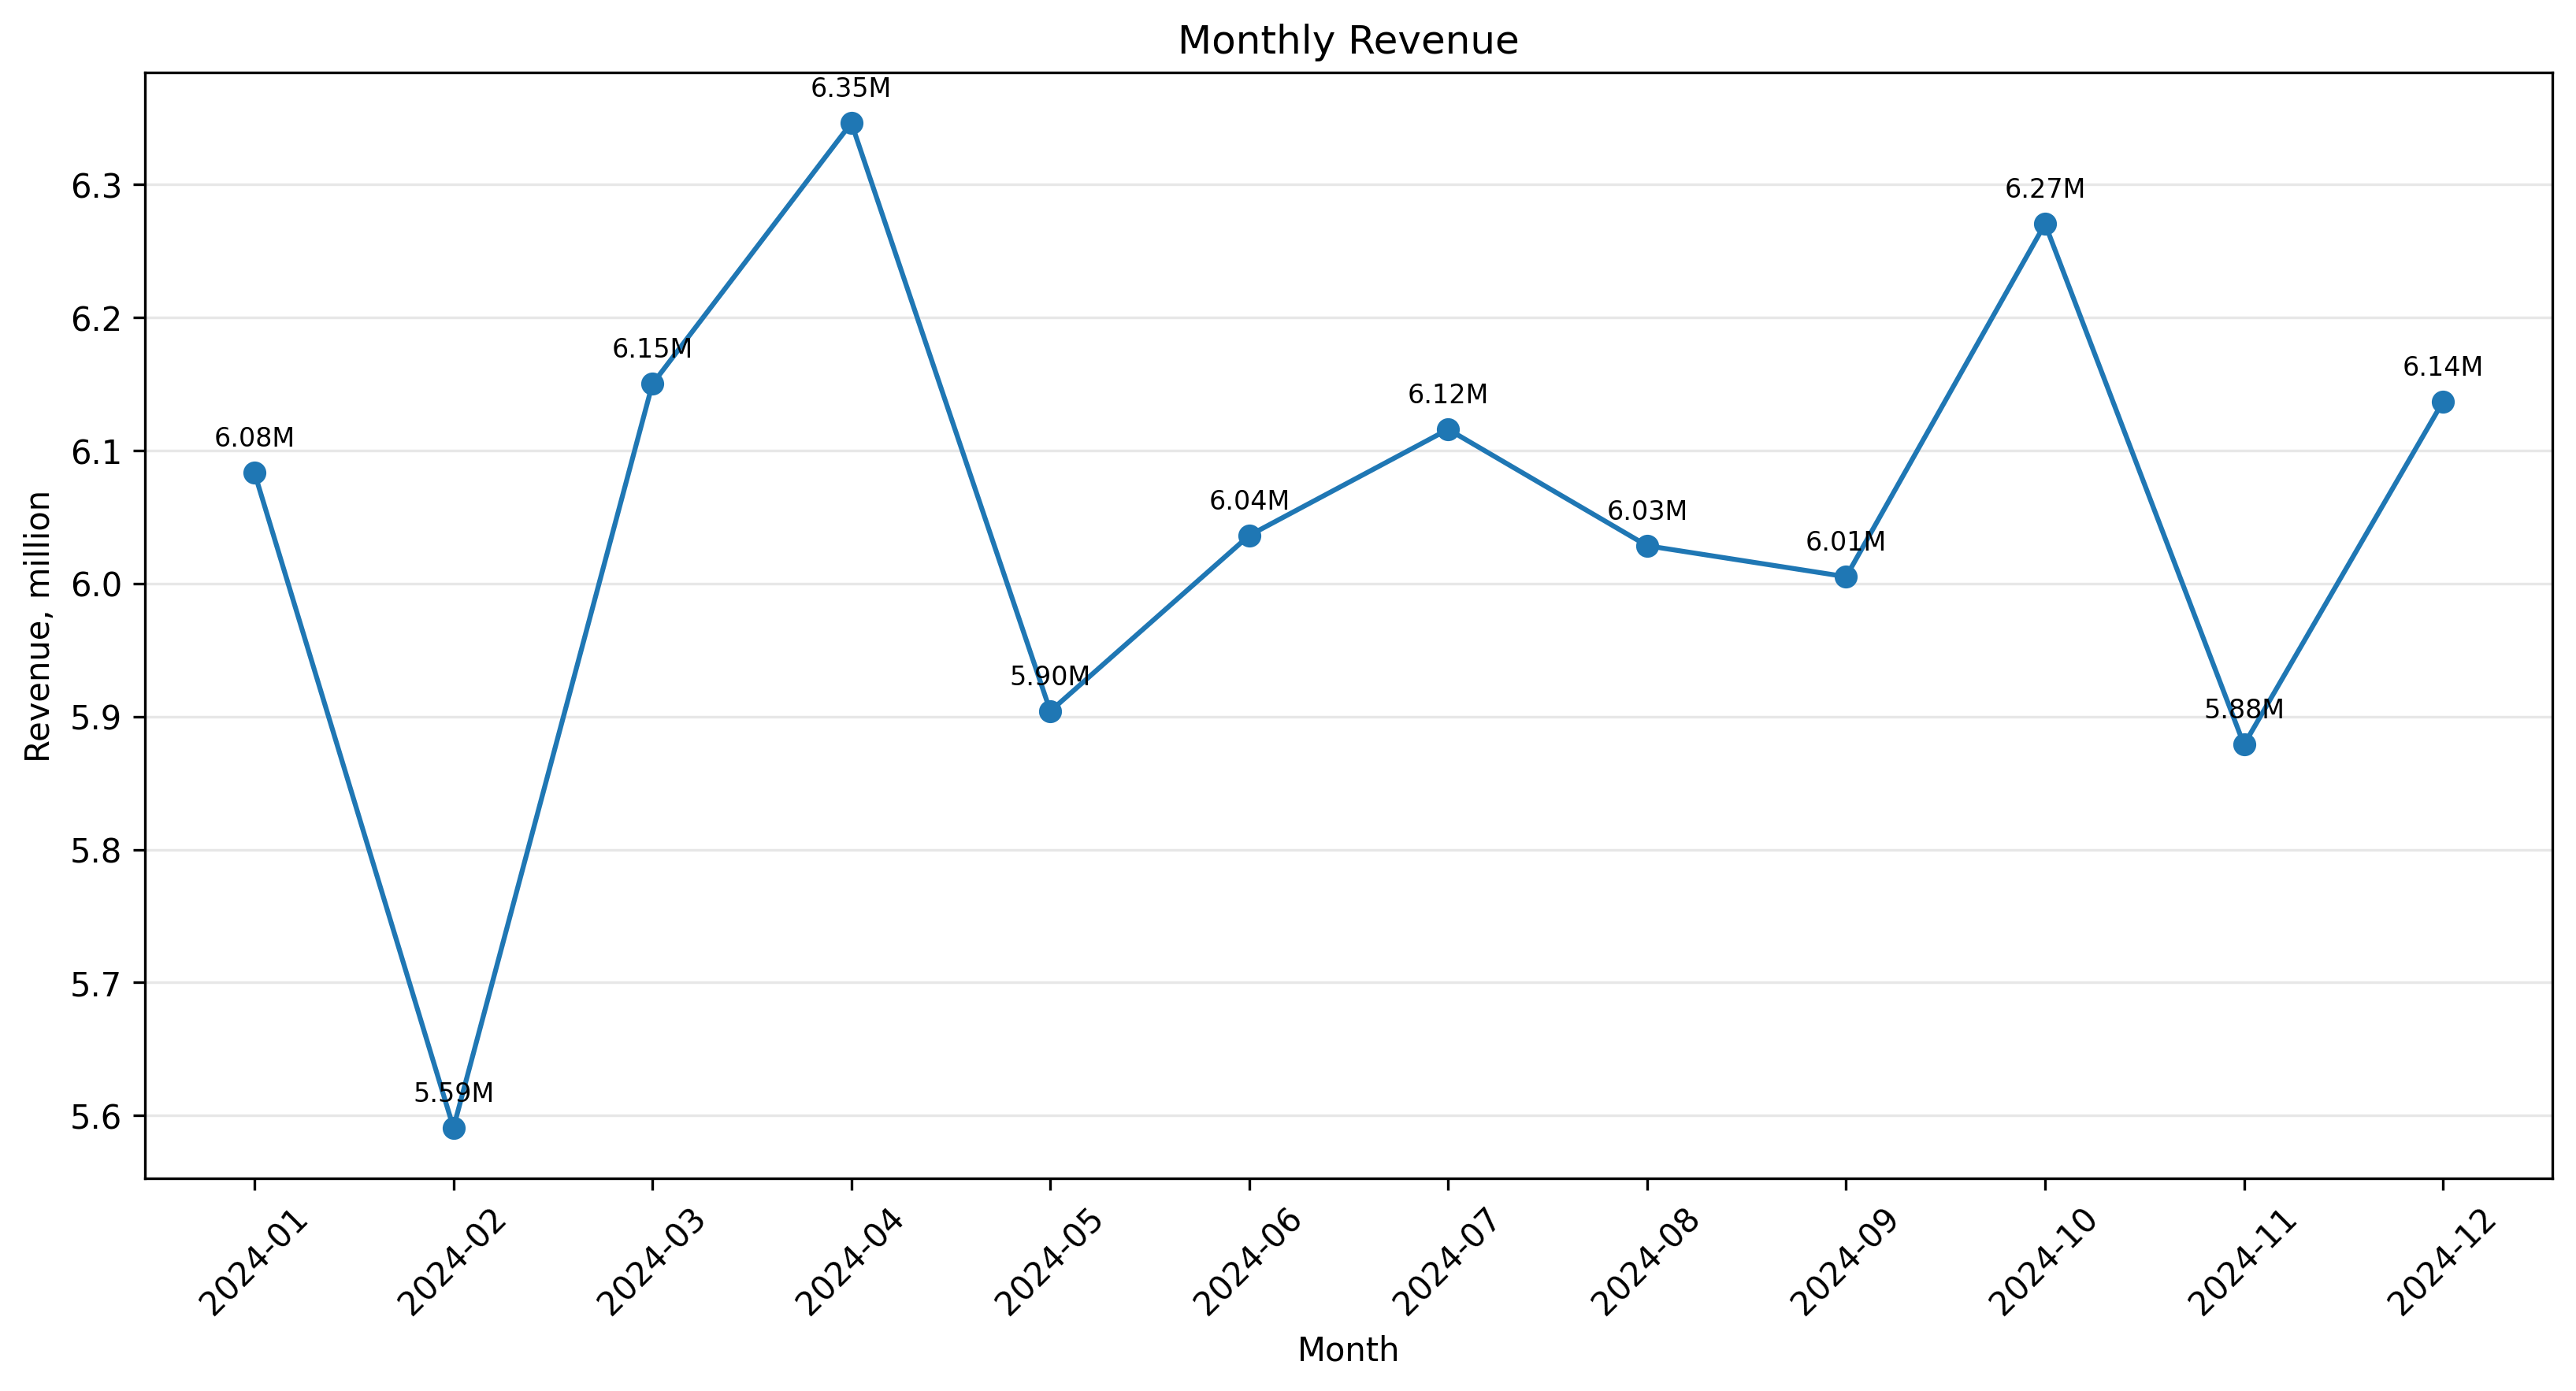
\includegraphics[
        width=0.95\textwidth
    ]{monthly_revenue.png}
    \caption{Динамика месячной выручки}
\end{figure}

\newpage
% ---------------------------------------------------------
\subsection{Количество покупок}
% ---------------------------------------------------------

Количество покупок менялось от 1~968 до 2~224 в месяц.

Минимальное значение было зафиксировано в феврале, максимальное ---
в октябре. Снижение количества покупок в феврале, мае и ноябре
совпадает со снижением выручки в эти месяцы.

\begin{figure}[H]
    \centering
    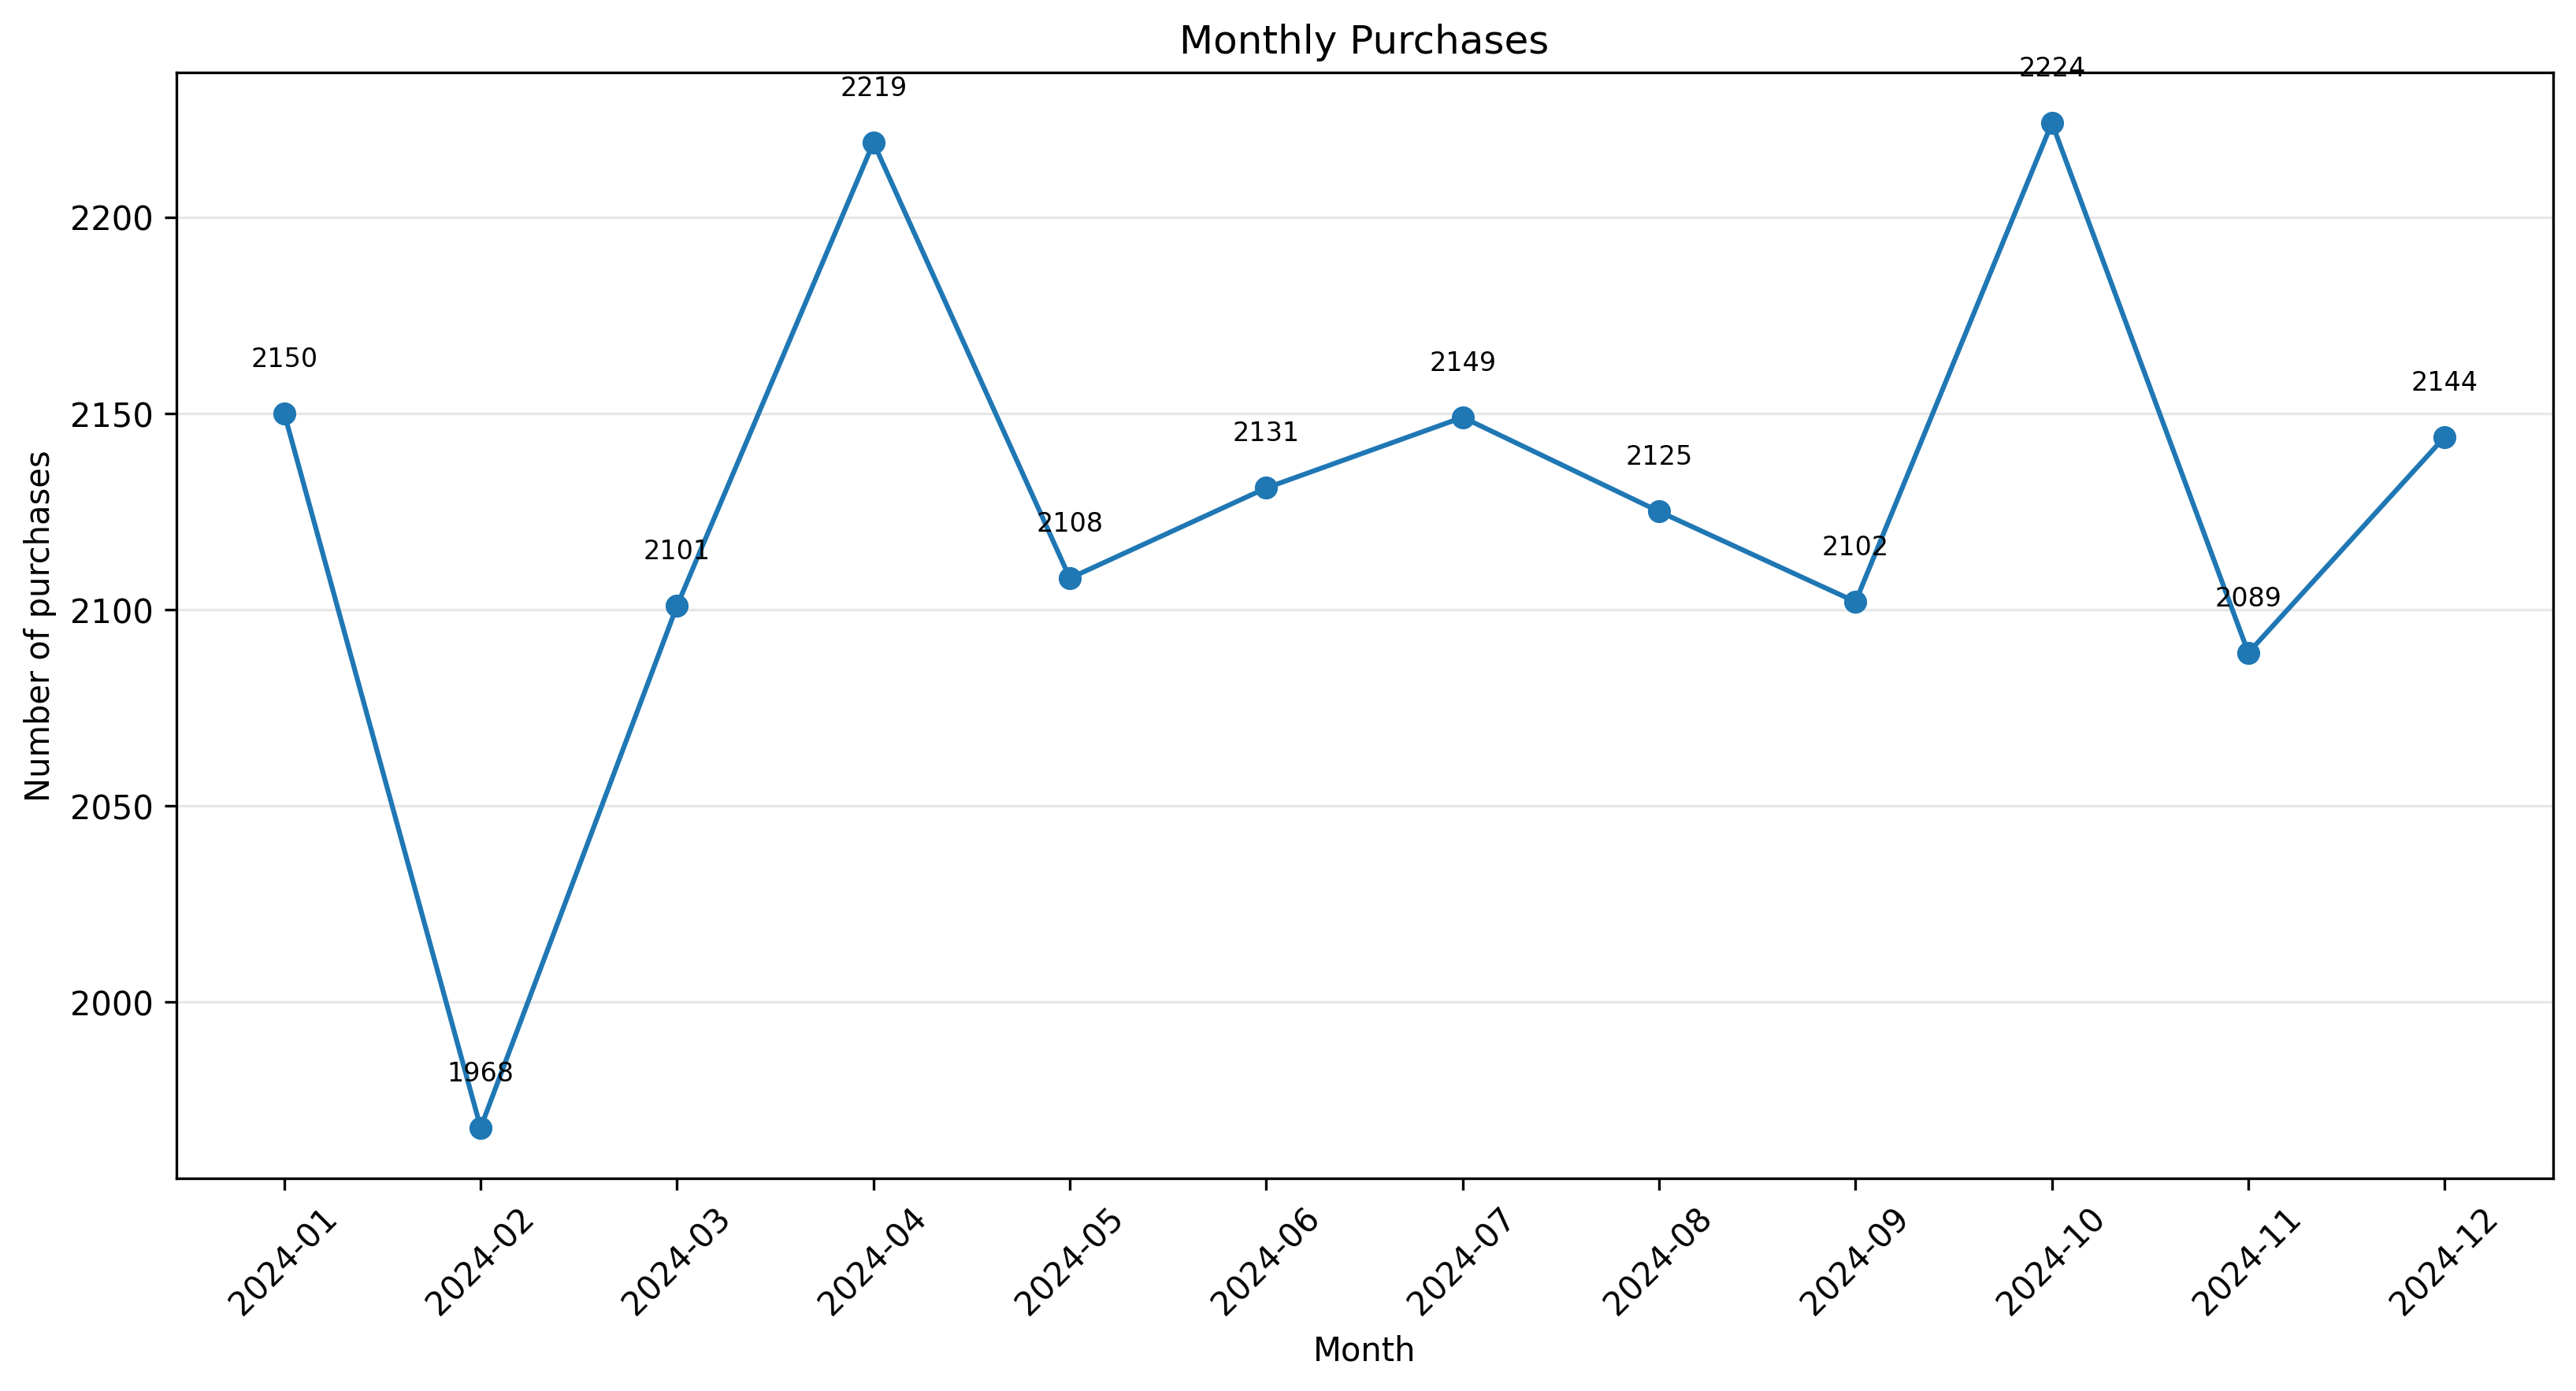
\includegraphics[
        width=0.95\textwidth
    ]{monthly_purchases.png}
    \caption{Количество покупок по месяцам}
\end{figure}

\newpage
% ---------------------------------------------------------
\subsection{Средний чек}
% ---------------------------------------------------------

Средний чек находился в диапазоне от 2~801 до 2~927.

Максимальное значение наблюдалось в марте, минимальное --- в мае.
Изменения среднего чека были менее выраженными, чем изменения
количества покупок.

\begin{figure}[H]
    \centering
    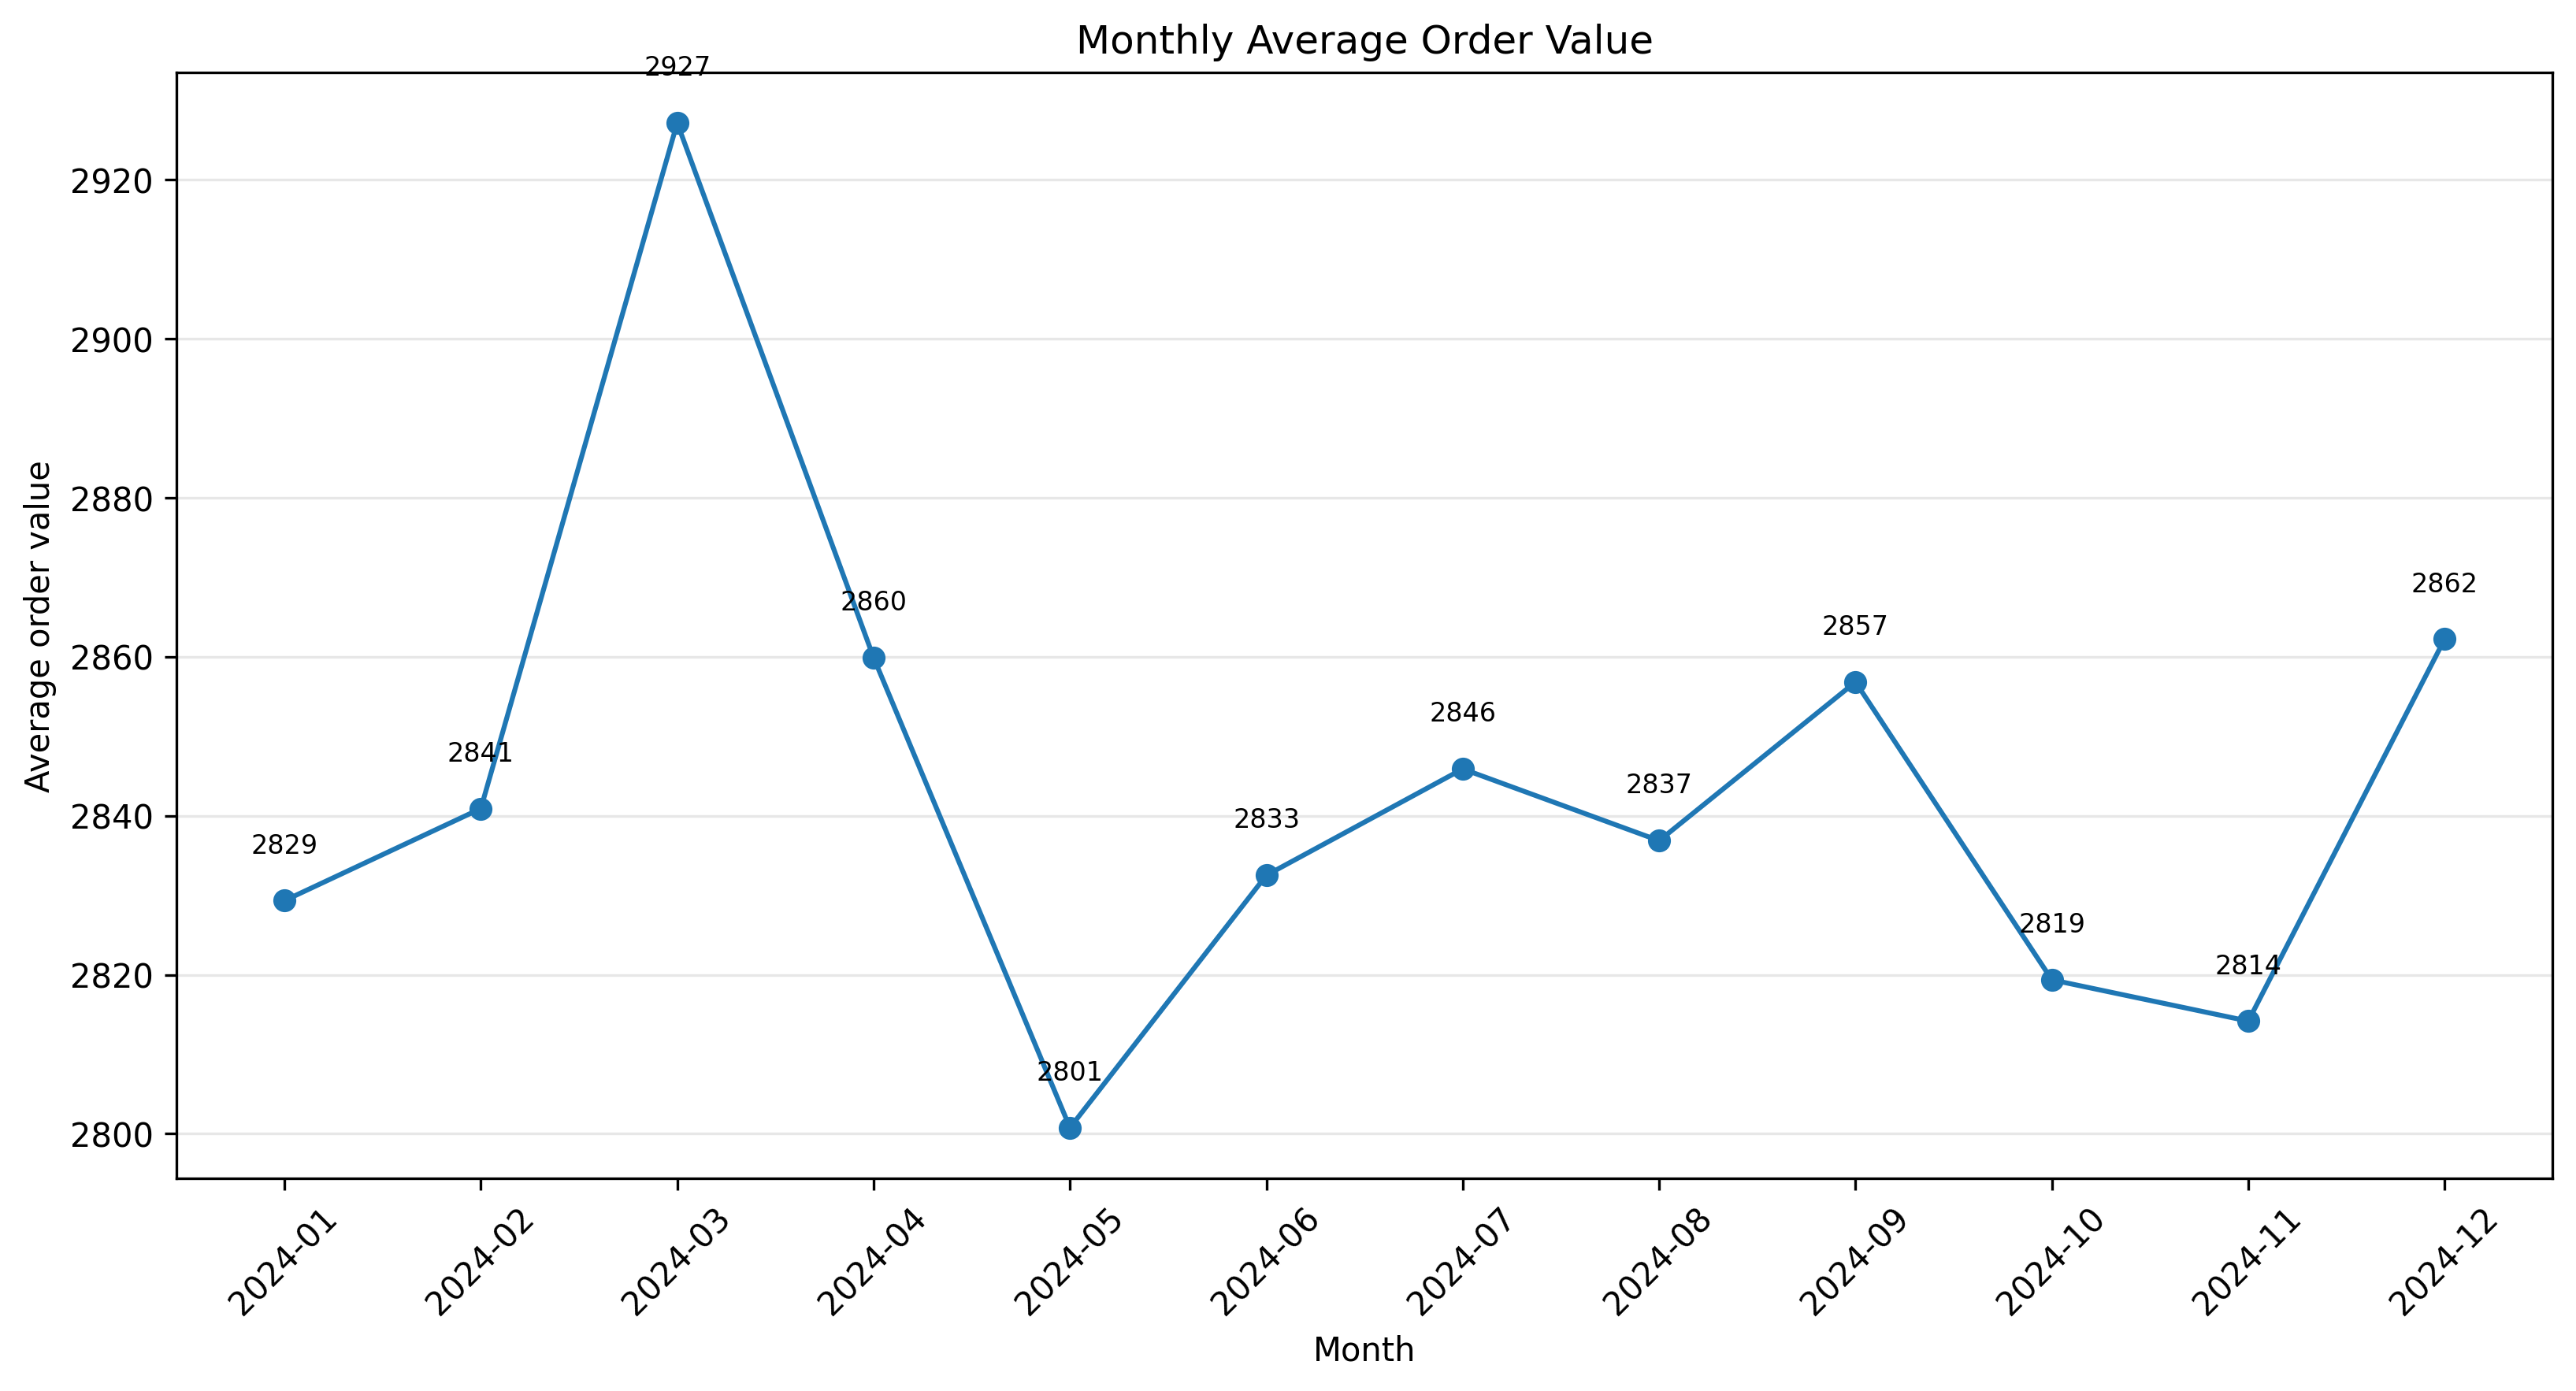
\includegraphics[
        width=0.95\textwidth
    ]{monthly_aov.png}
    \caption{Средний чек по месяцам}
\end{figure}

Таким образом, месячные колебания выручки в большей степени связаны
с количеством покупок, чем с изменением среднего чека.

\newpage
% ---------------------------------------------------------
\section{Анализ покупателей}
% ---------------------------------------------------------

Всего покупателями стали 10~566 пользователей.

Распределение по количеству покупок представлено в таблице.

\begin{table}[H]
    \centering
    \caption{Распределение покупателей по количеству покупок}
    \begin{tabular}{ccc}
        \toprule
        Покупок & Покупателей & Доля, \% \\
        \midrule
        1  & 3~052 & 28,89 \\
        2  & 3~172 & 30,02 \\
        3  & 2~362 & 22,35 \\
        4  & 1~201 & 11,37 \\
        5  & 534   & 5,05 \\
        6  & 178   & 1,68 \\
        7  & 53    & 0,50 \\
        8  & 12    & 0,11 \\
        9  & 1     & 0,01 \\
        10 & 1     & 0,01 \\
        \bottomrule
    \end{tabular}
\end{table}

Наиболее многочисленная группа --- пользователи с двумя покупками.
Около 81,3\% покупателей совершили не более трёх покупок.

\begin{figure}[H]
    \centering
    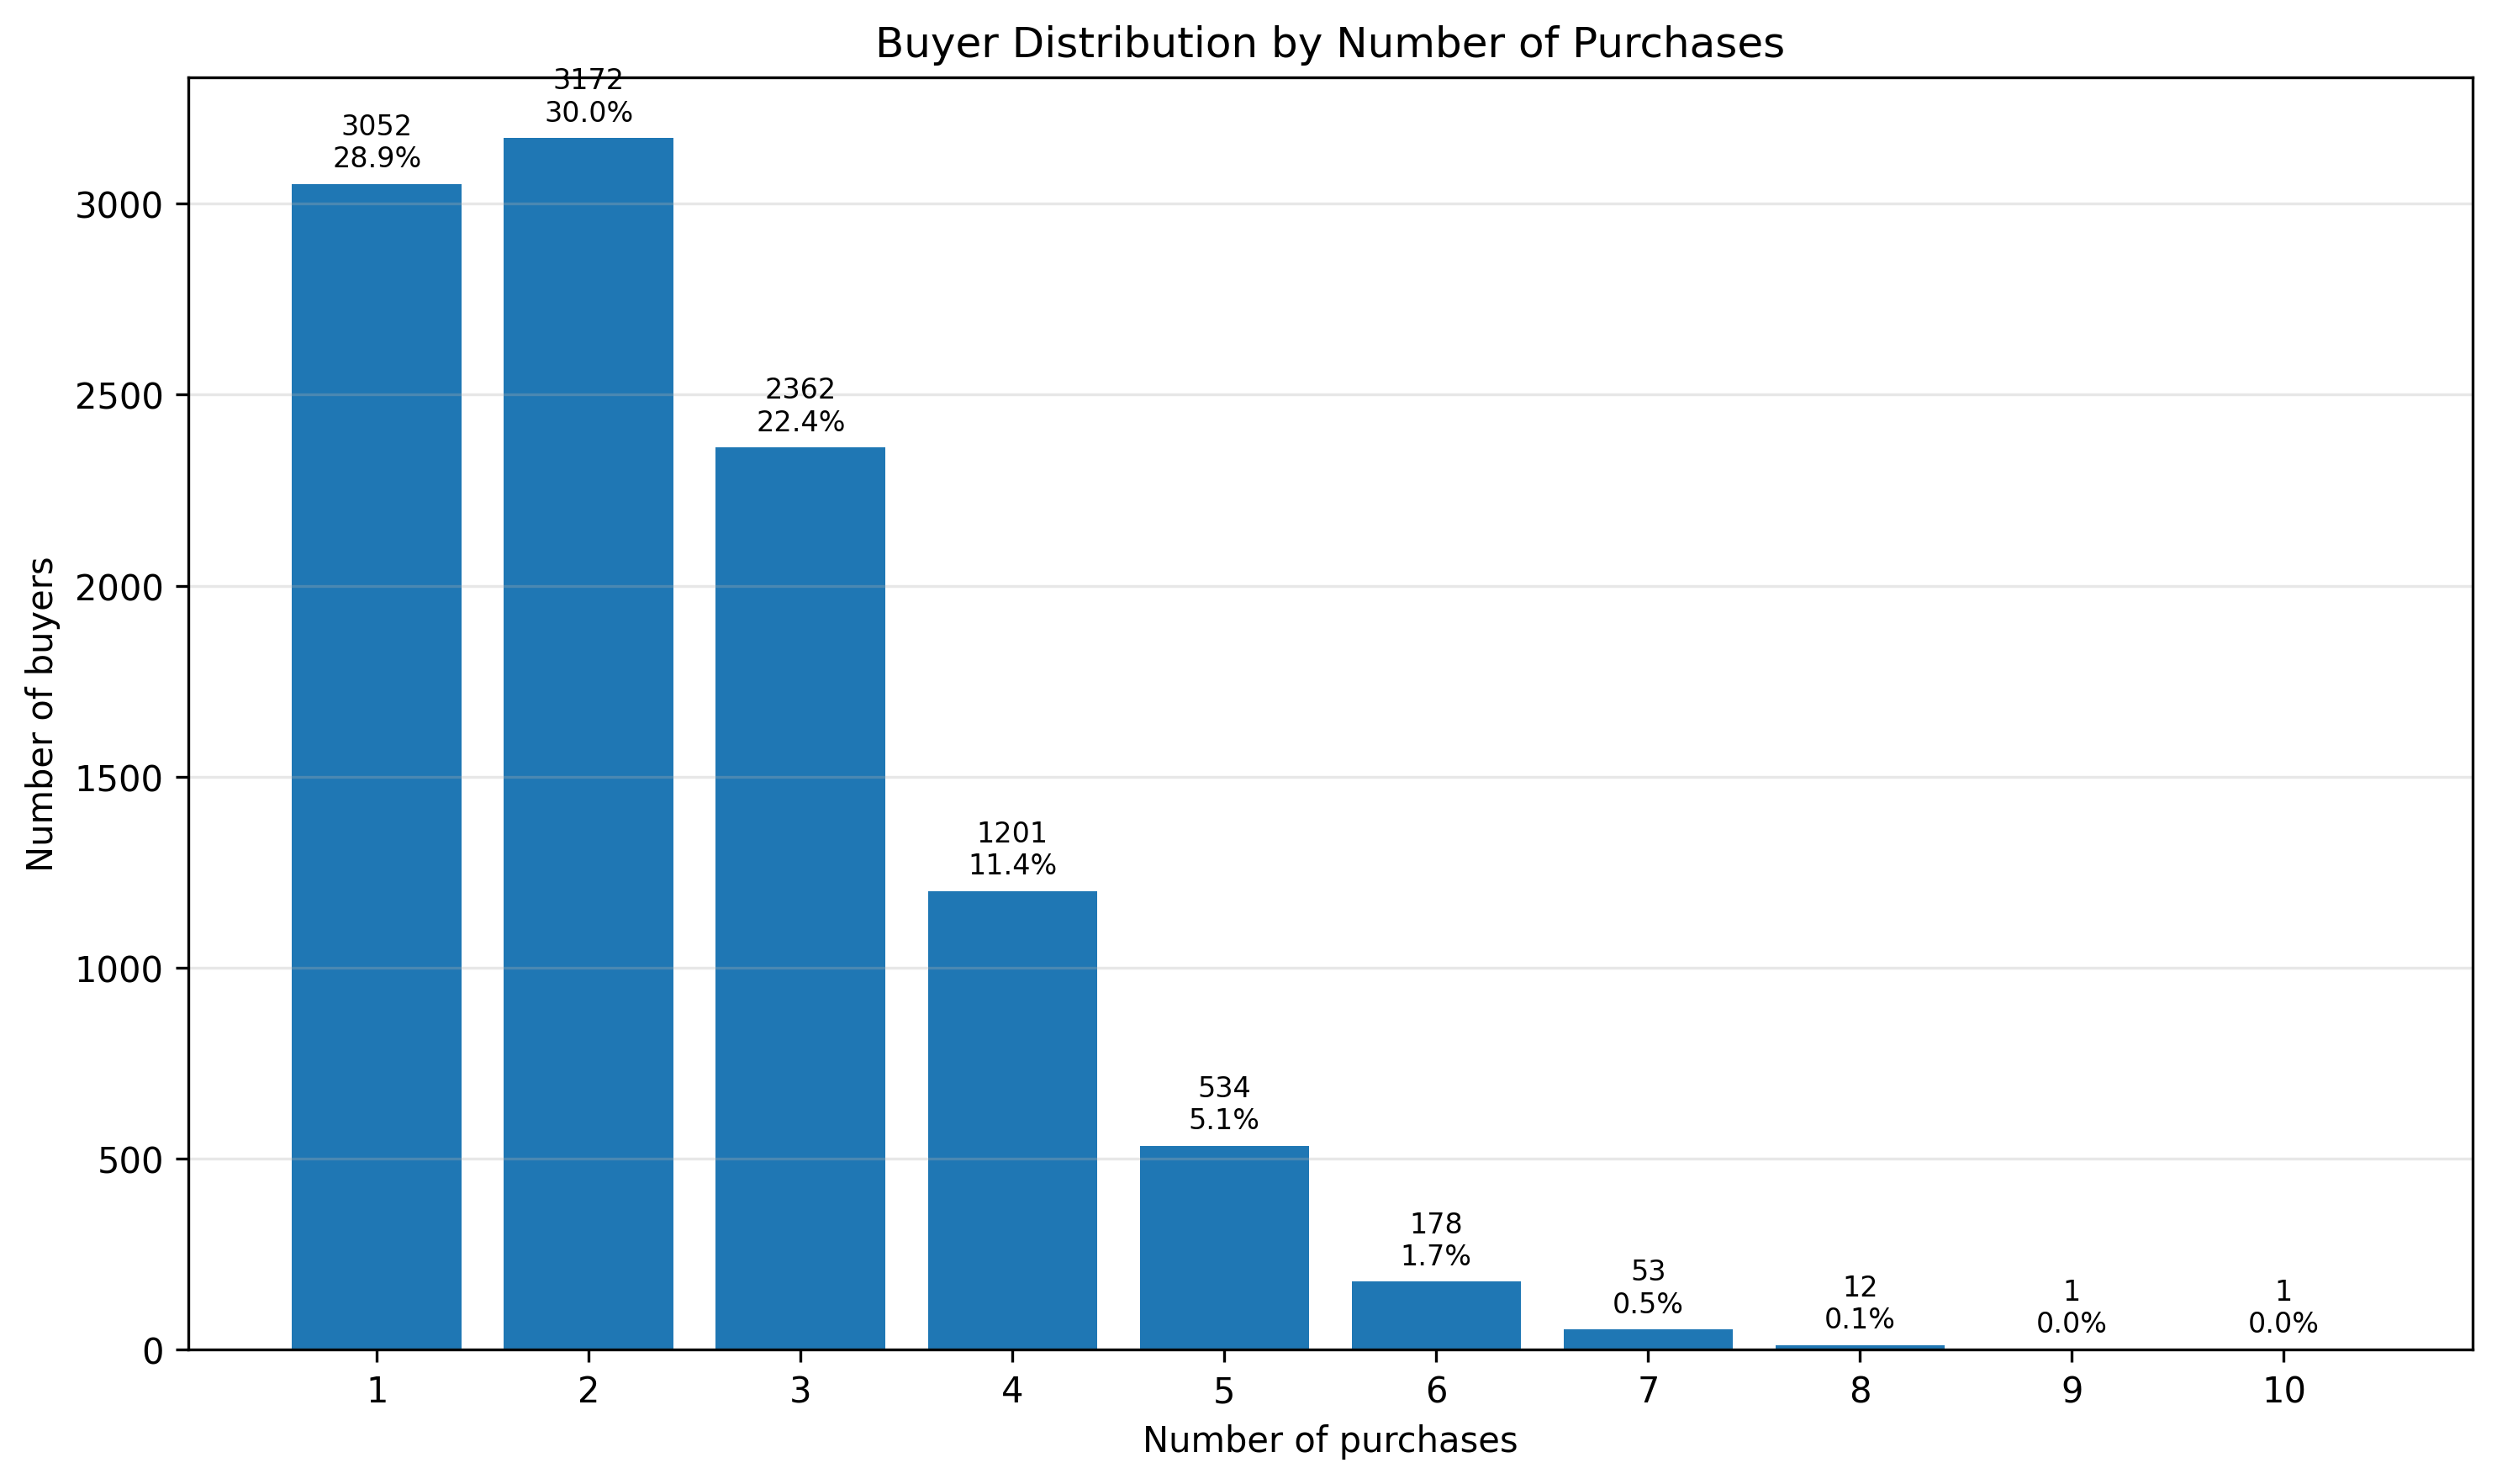
\includegraphics[
        width=0.95\textwidth
    ]{buyers_by_purchase_count.png}
    \caption{Распределение покупателей по количеству покупок}
\end{figure}

% ---------------------------------------------------------
\subsection{Разовые и повторные покупатели}
% ---------------------------------------------------------

Разовыми считались пользователи, совершившие одну покупку.
К повторным были отнесены пользователи с двумя покупками и более.

\begin{table}[H]
    \centering
    \caption{Показатели по типу покупателя}
    \begin{tabular}{lrrrr}
        \toprule
        Тип &
        Покупатели &
        Покупки &
        Выручка, млн &
        Доля выручки, \% \\
        \midrule
        Разовые &
        3~052 &
        3~052 &
        8,63 &
        11,90 \\
        Повторные &
        7~514 &
        22~458 &
        63,91 &
        88,10 \\
        \bottomrule
    \end{tabular}
\end{table}

Повторные покупатели составляют 71,1\% покупателей и формируют
88,1\% всей выручки.

Средняя выручка на одного повторного покупателя примерно в три раза
выше, чем на одного разового покупателя.

Этот результат является описательной связью. Он не доказывает,
что увеличение количества повторных покупок автоматически вызовет
пропорциональный рост выручки.

\begin{figure}[H]
    \centering
    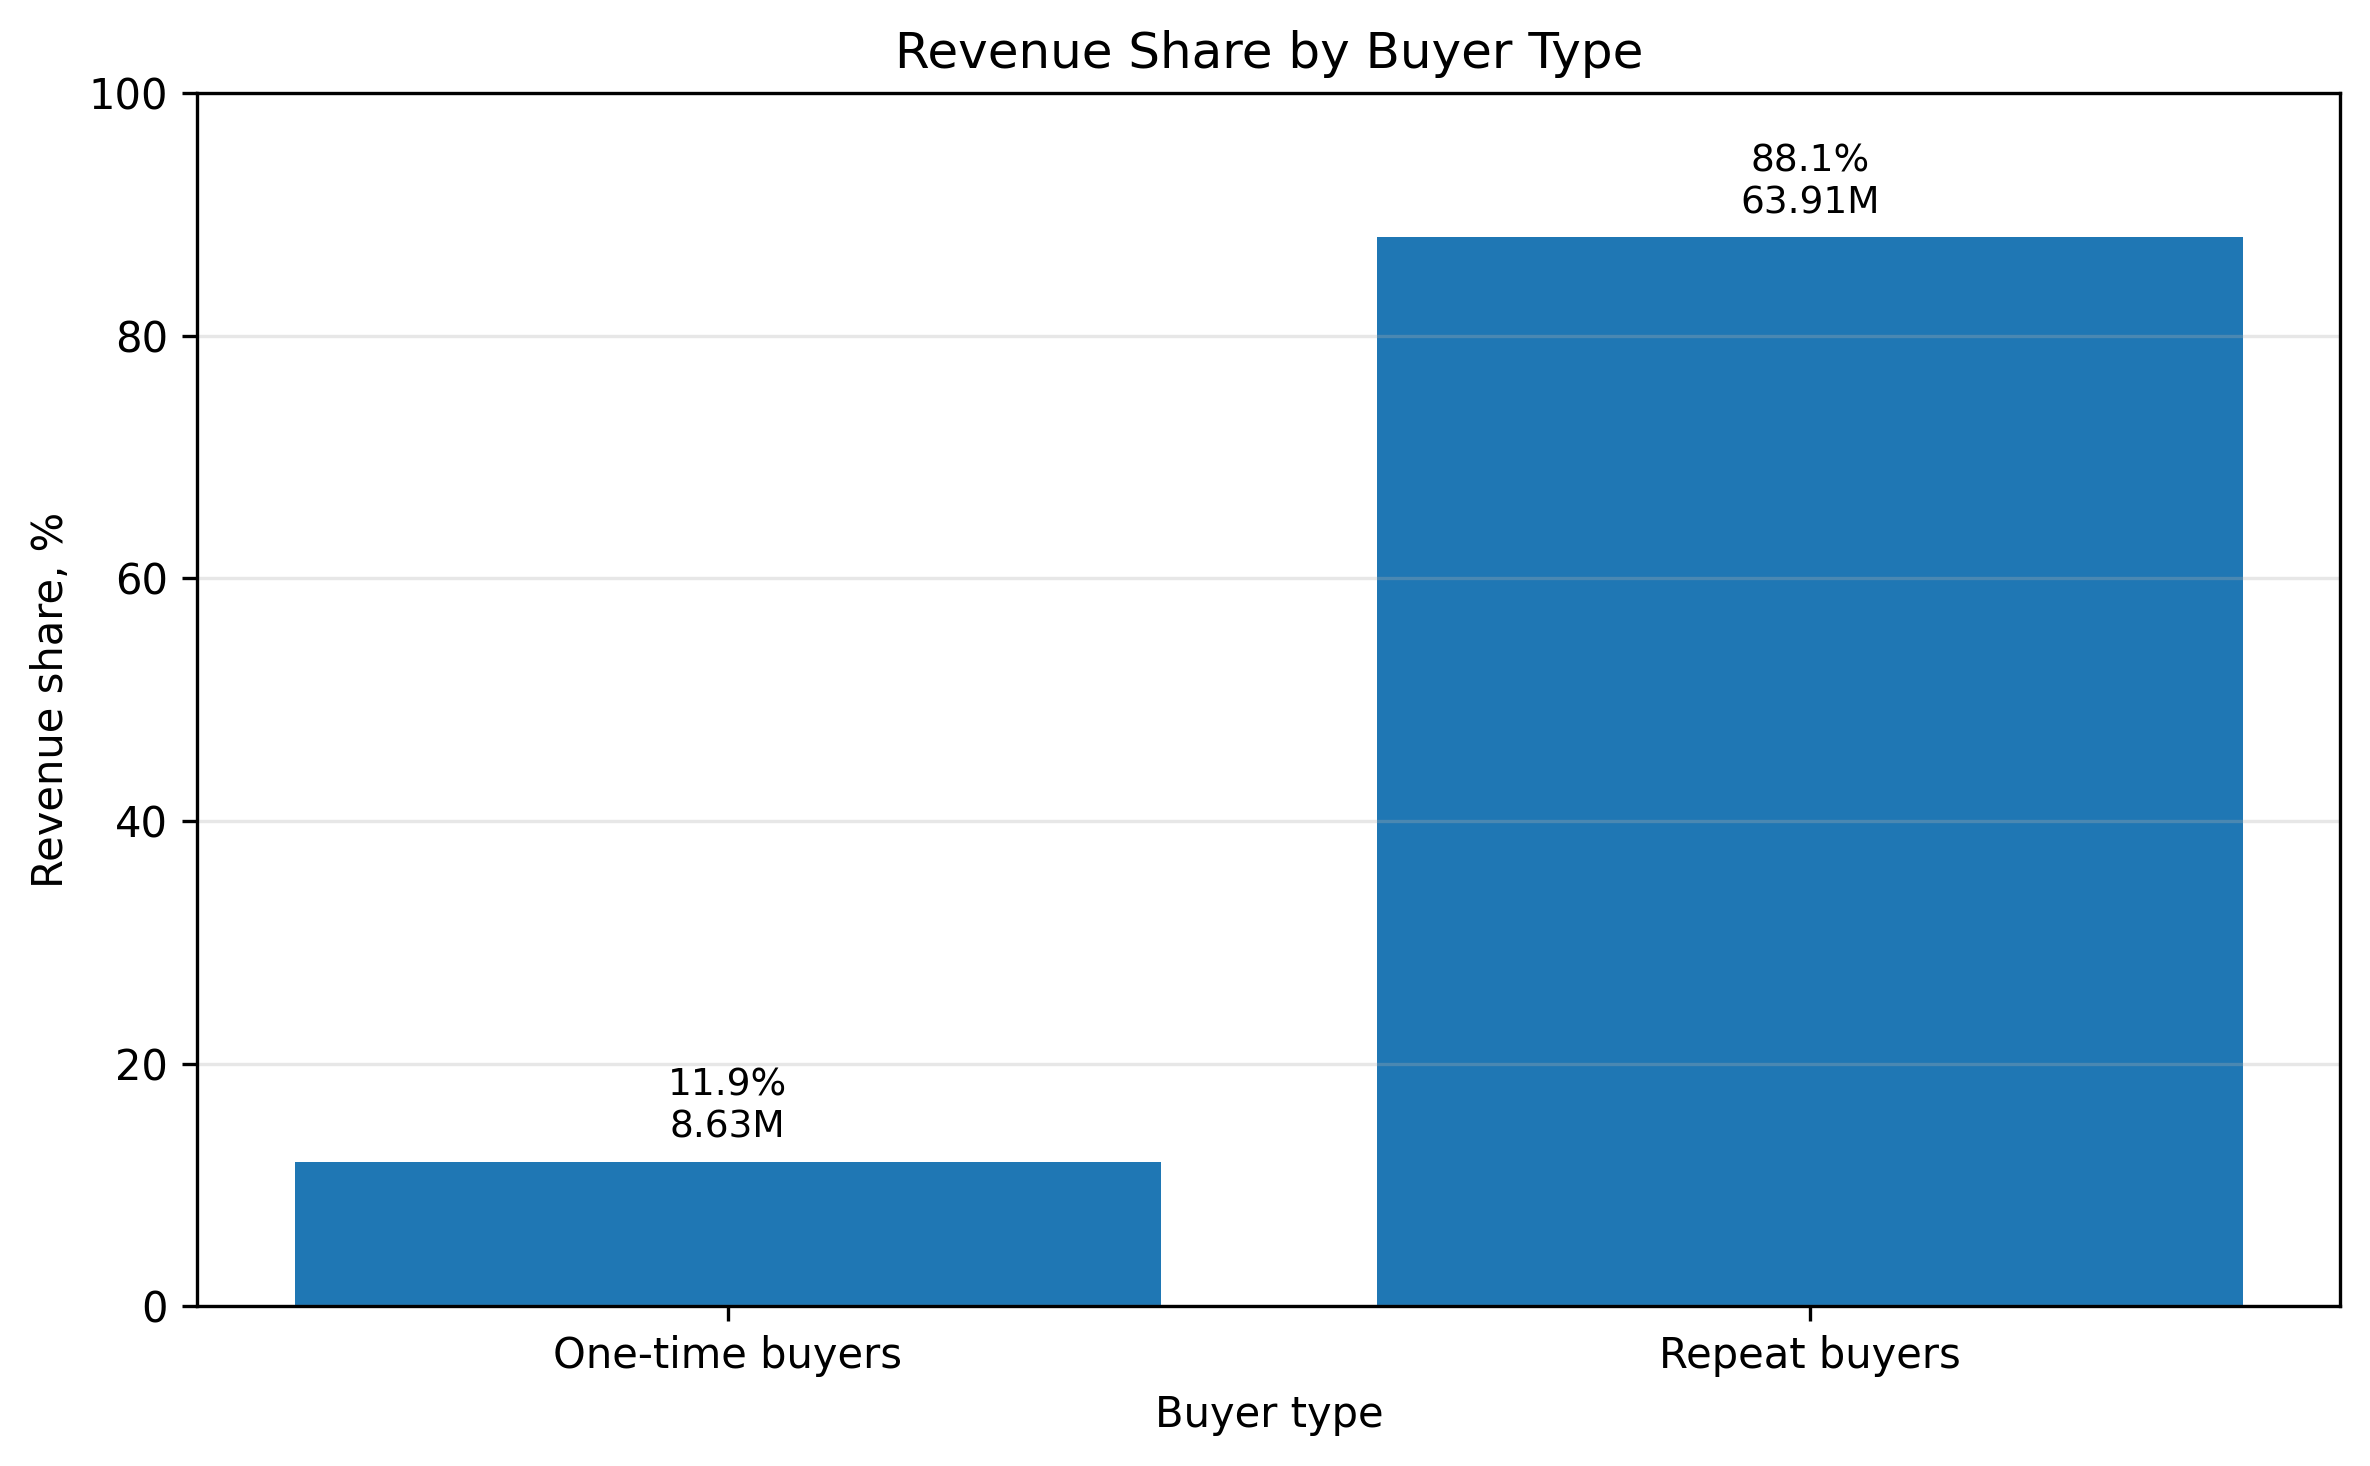
\includegraphics[
        width=0.9\textwidth
    ]{revenue_share_by_buyer_type.png}
    \caption{Доля выручки разовых и повторных покупателей}
\end{figure}

\newpage
% ---------------------------------------------------------
\section{Время до второй покупки}
% ---------------------------------------------------------

Для каждого повторного покупателя был рассчитан интервал между первой
и второй покупкой.

Среднее время до второй покупки составило 99,96 дня, медианное ---
81 день.

\begin{table}[H]
    \centering
    \caption{Срок совершения второй покупки}
    \begin{tabular}{lrr}
        \toprule
        Период & Покупателей & Доля, \% \\
        \midrule
        В тот же день    & 30    & 0,40 \\
        1--7 дней        & 384   & 5,11 \\
        8--30 дней       & 1~242 & 16,53 \\
        31--60 дней      & 1~319 & 17,55 \\
        61--90 дней      & 1~116 & 14,85 \\
        Более 90 дней    & 3~423 & 45,55 \\
        \bottomrule
    \end{tabular}
\end{table}

В течение 30 дней вторую покупку совершили 22,04\% повторных
покупателей. В течение 90 дней вернулись 54,45\%.

Почти половина повторных покупателей совершила вторую покупку позднее
чем через 90 дней. Поэтому короткое окно наблюдения может заметно
занижать оценку повторных покупок.

\begin{figure}[H]
    \centering
    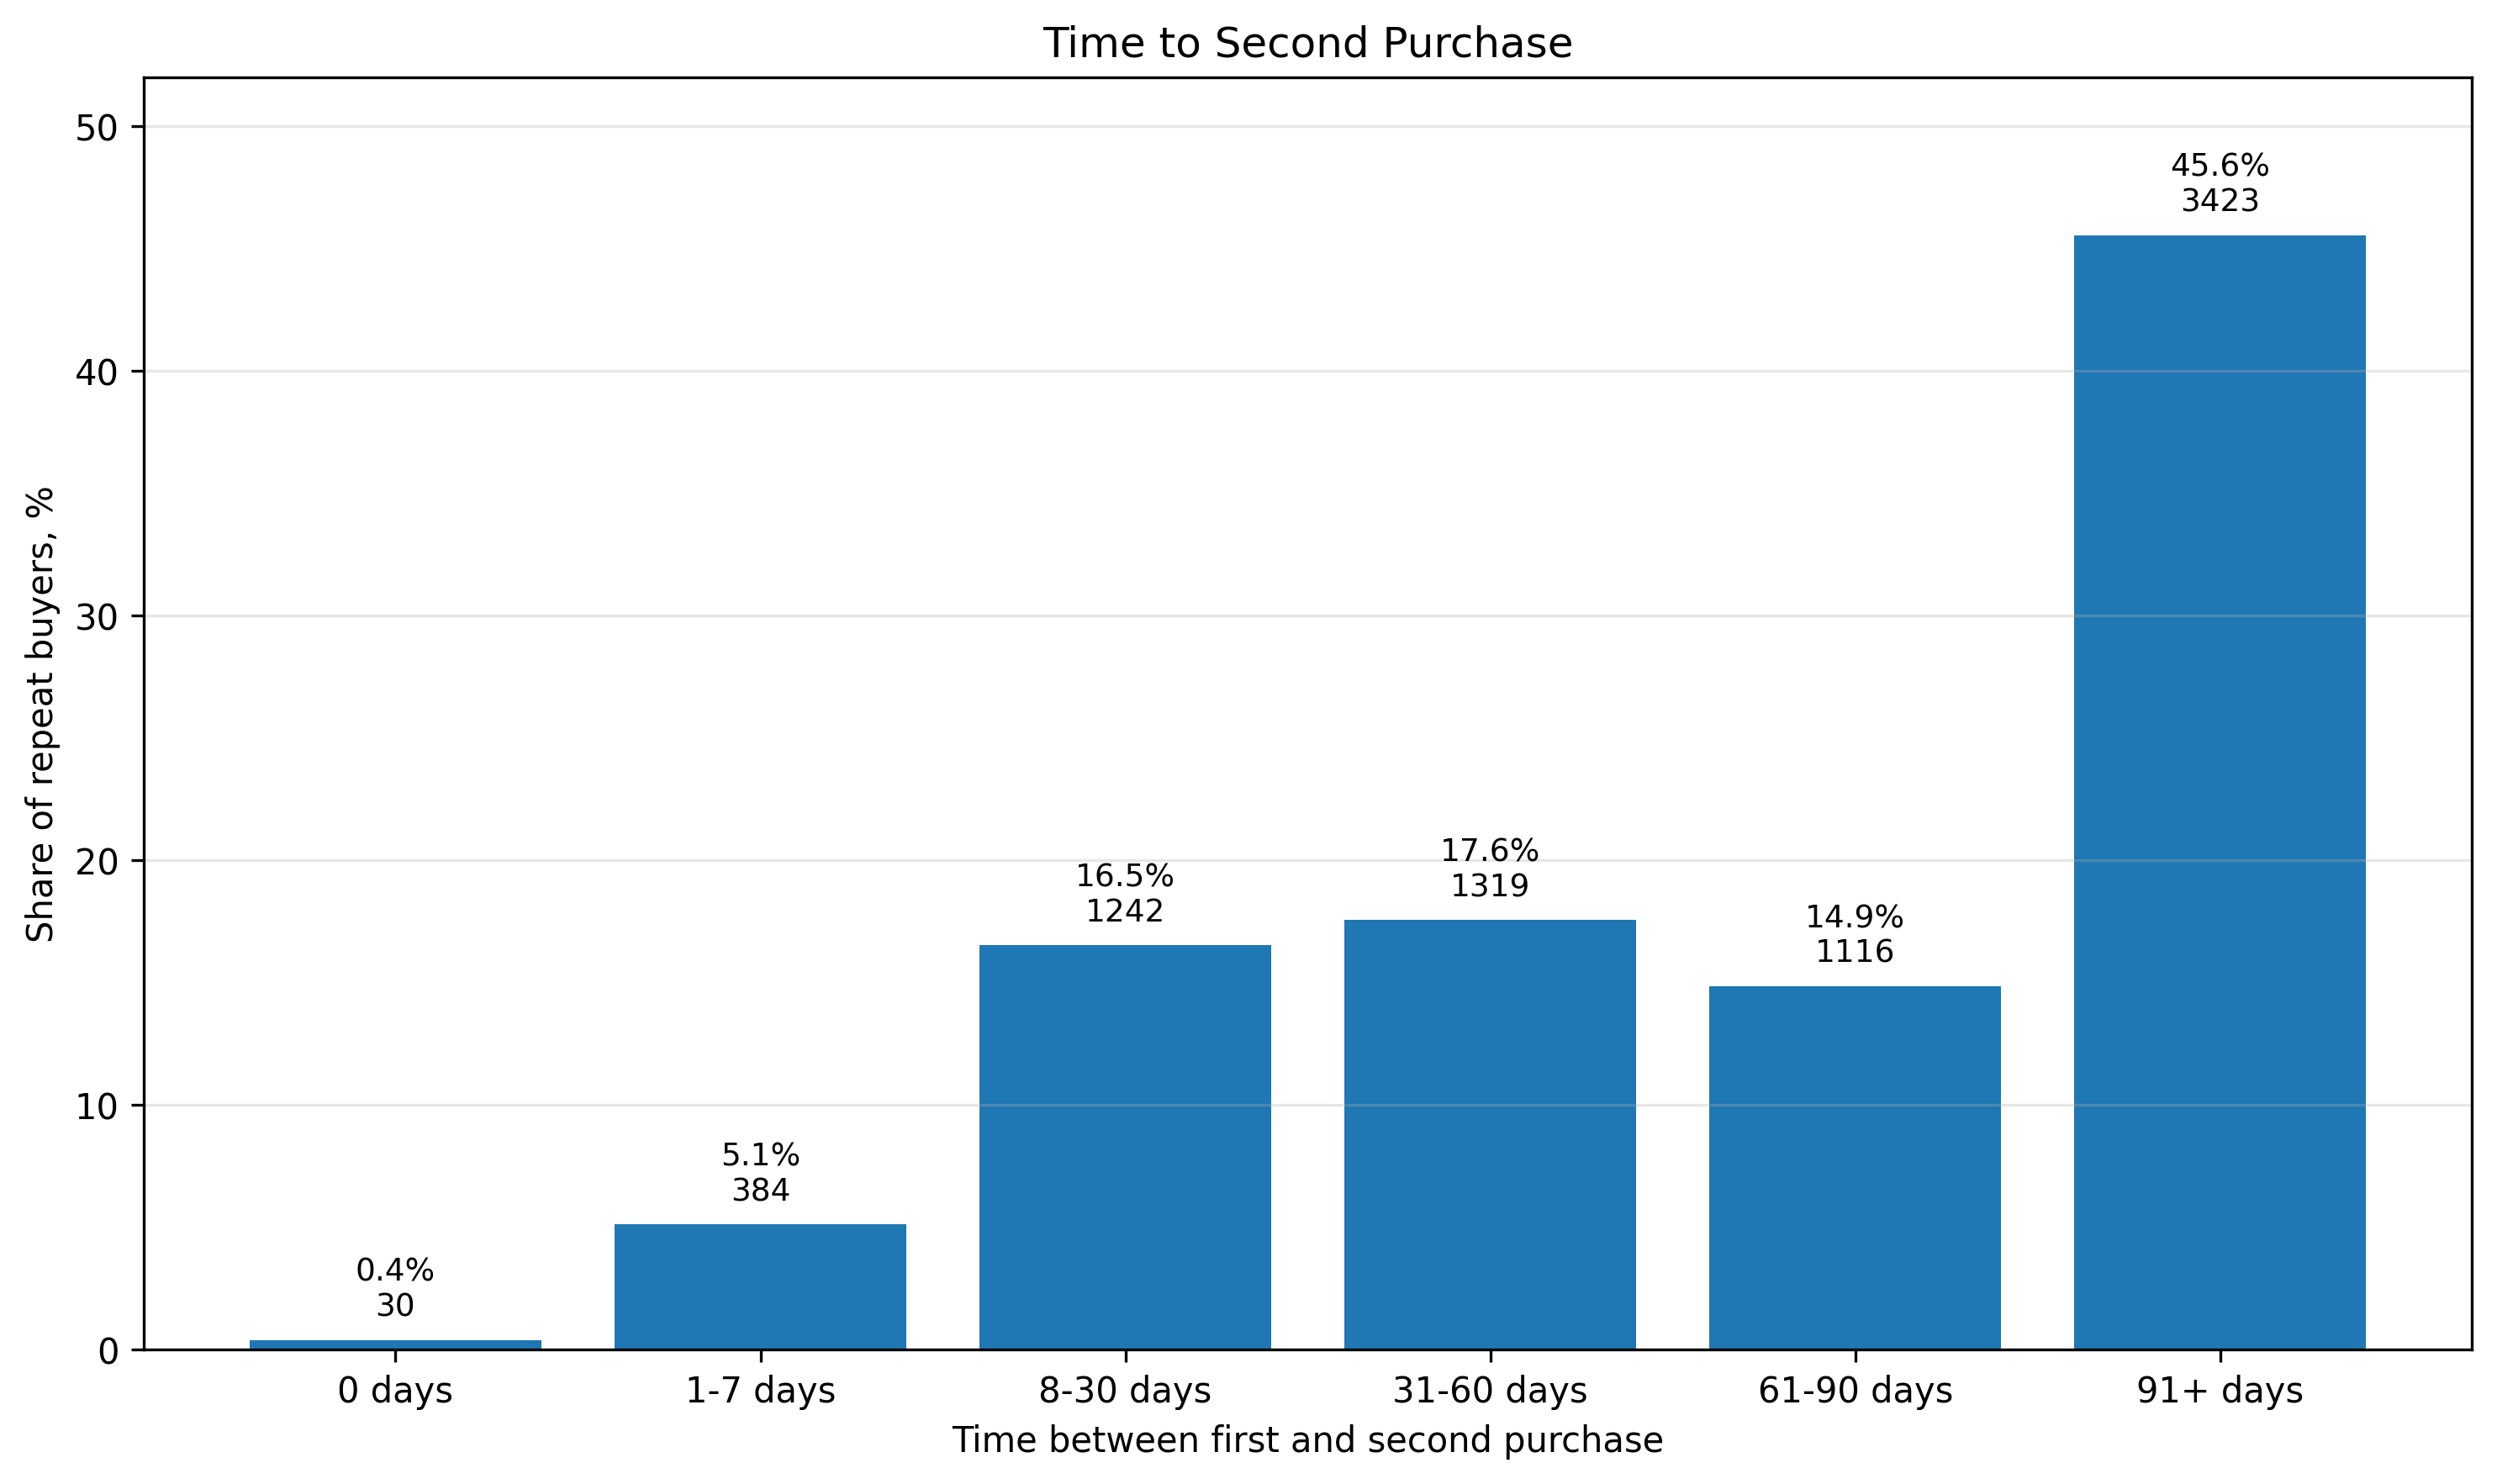
\includegraphics[
        width=0.95\textwidth
    ]{repeat_purchase_interval.png}
    \caption{Распределение времени до второй покупки}
\end{figure}

% ---------------------------------------------------------
\section{Когортный анализ}
% ---------------------------------------------------------

Покупатели были разделены на когорты по месяцу первой покупки.

Для каждой когорты рассчитывалась доля пользователей, совершивших
покупку в последующие календарные месяцы:

\[
\text{Retention}_{m}
=
\frac{
    \text{Активные покупатели когорты в месяце } m
}{
    \text{Размер когорты}
}
\cdot 100\%.
\]

Месяц первой покупки обозначен как \(M0\), следующий календарный
месяц --- как \(M1\), далее \(M2\), \(M3\) и так далее.

В большинстве когорт месячный retention находился примерно в диапазоне
14--18\%. Выраженного улучшения или ухудшения показателя между
когортами не обнаружено.

\begin{figure}[H]
    \centering
    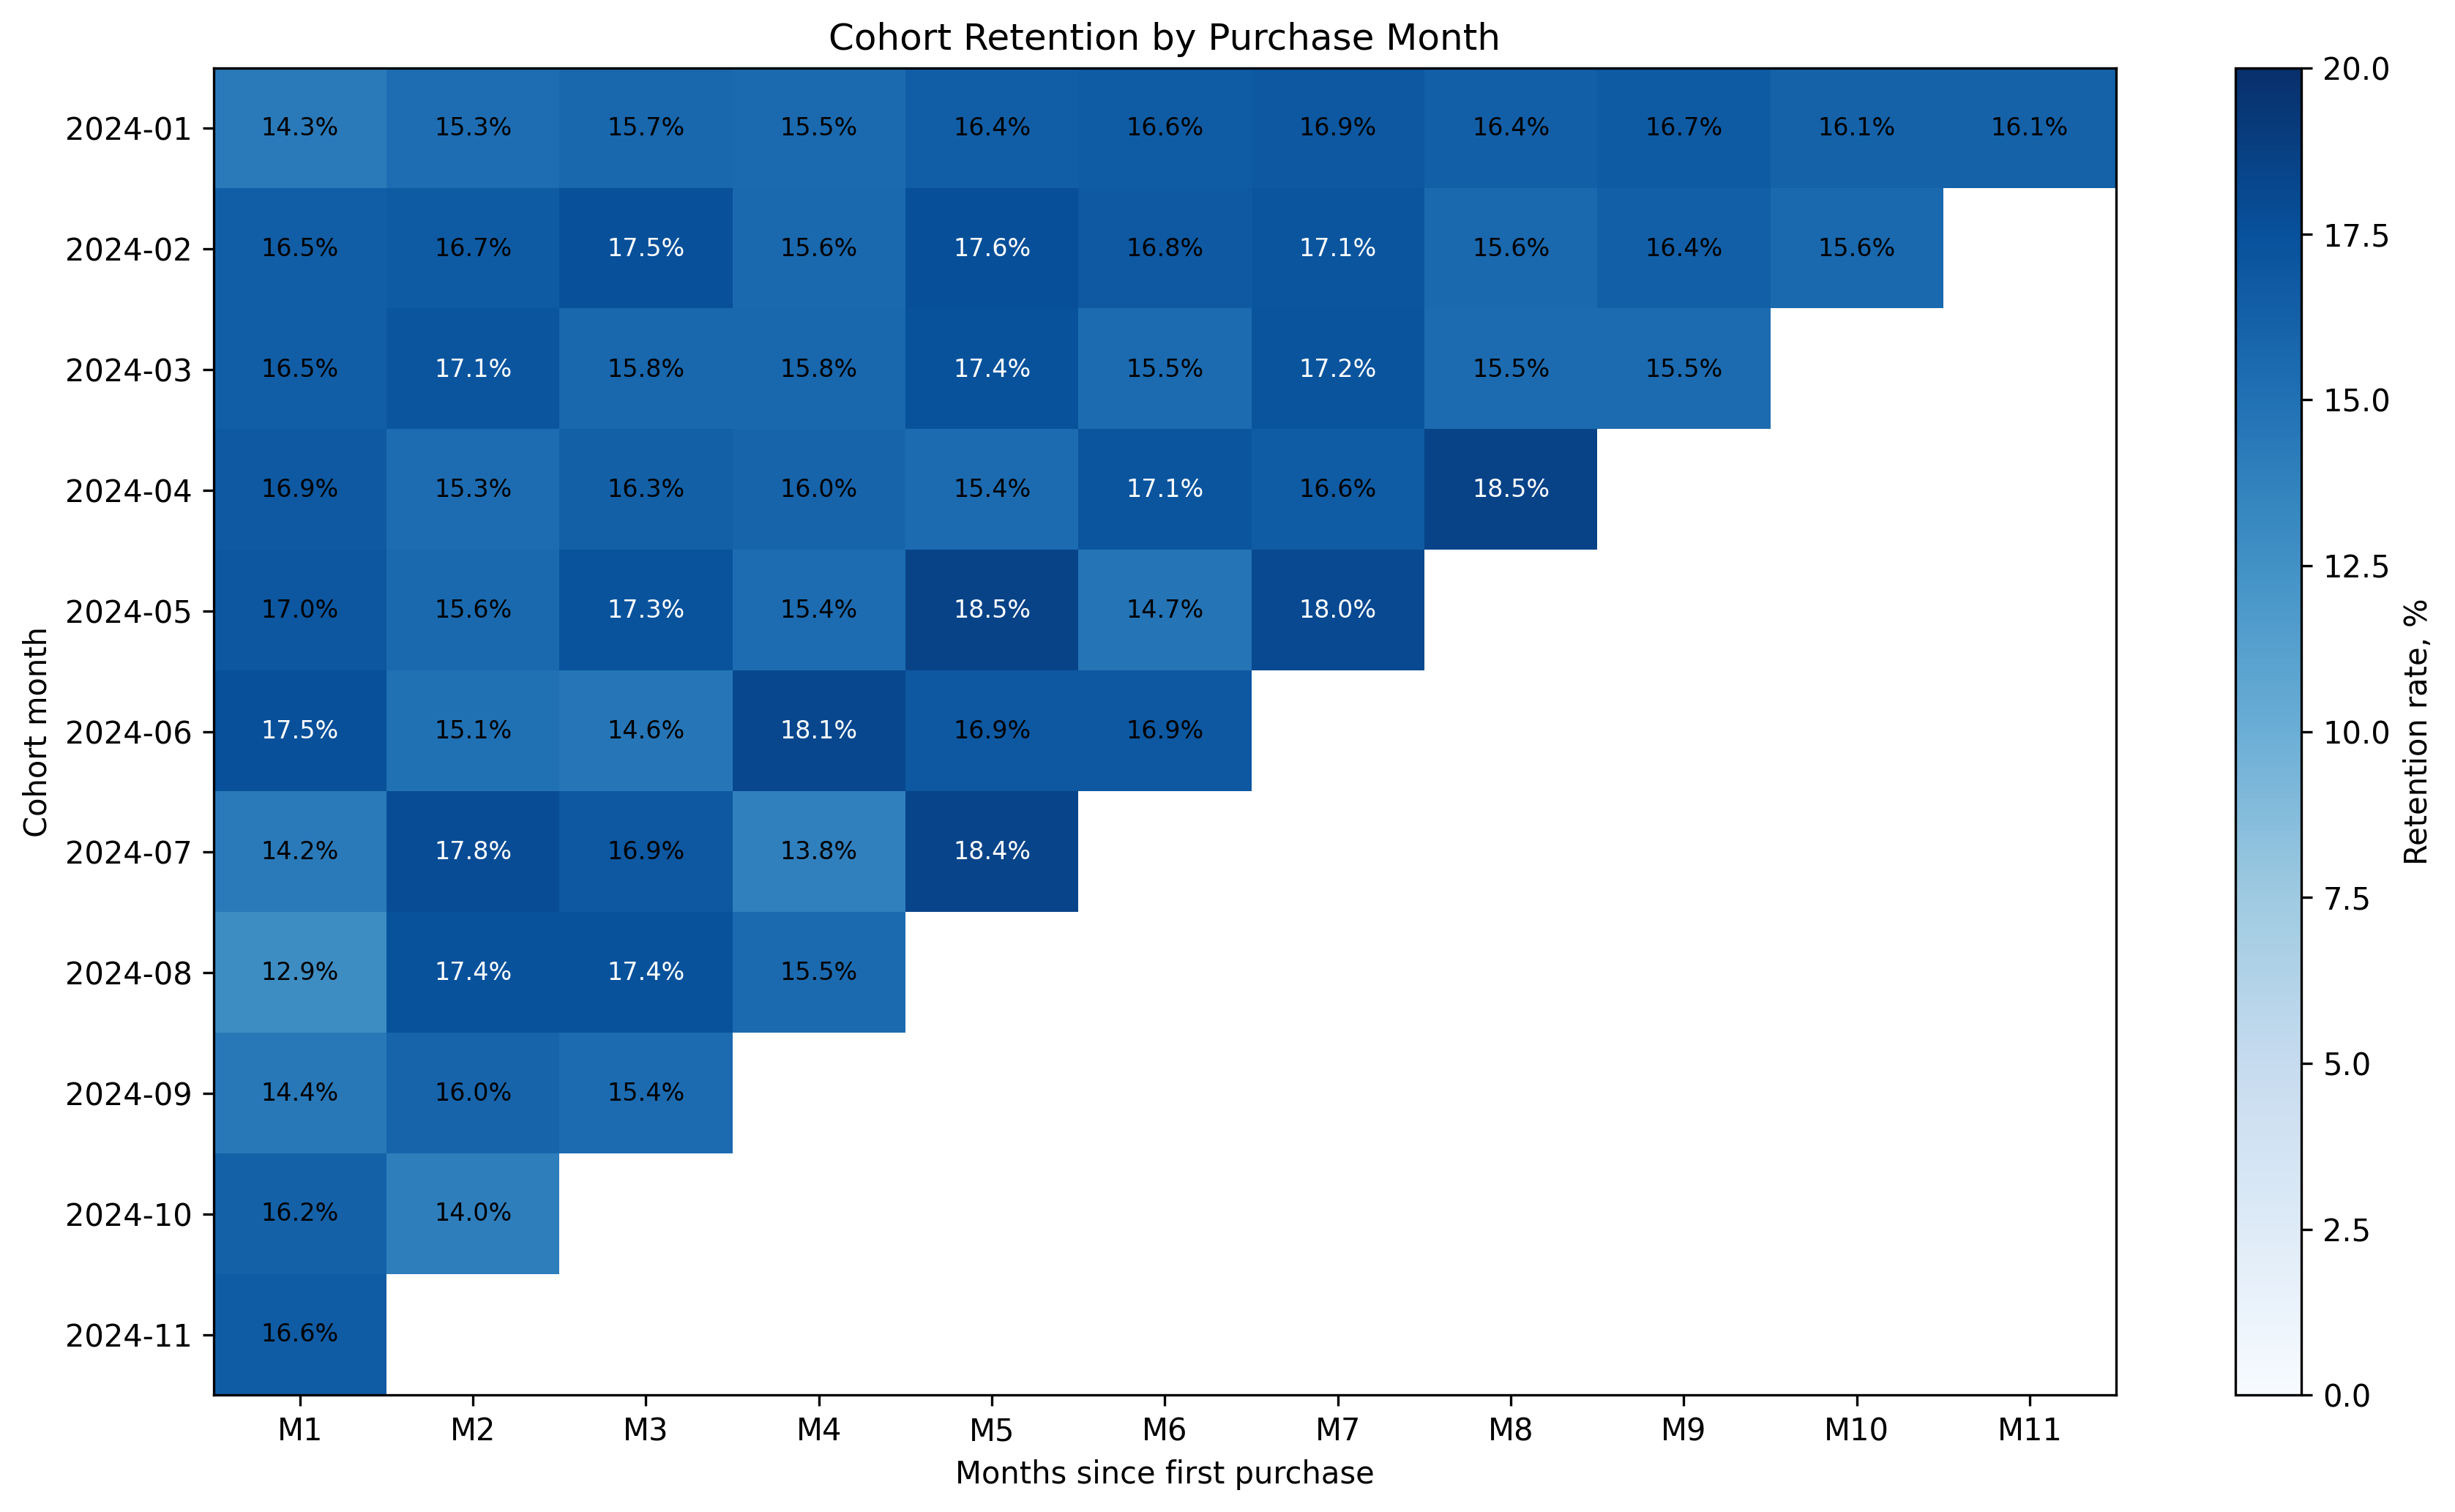
\includegraphics[
        width=0.95\textwidth
    ]{cohort_retention_heatmap.png}
    \caption{Когортный retention покупателей}
\end{figure}

Пустые ячейки в правой части графика не означают нулевой retention.
Соответствующие периоды отсутствуют из-за окончания наблюдаемого
интервала.

Покупатели, совершившие первую покупку в конце года, имели меньше
времени для повторной активности. Это ограничение необходимо учитывать
при сравнении когорт.

\newpage
% ---------------------------------------------------------
\section{A/B-тест}
% ---------------------------------------------------------

В эксперименте сравнивались старая и новая версии посадочной страницы.

Контрольная группа видела старую страницу, тестовая группа ---
новую страницу.

Нулевая гипотеза:

\[
H_0:
p_{\text{treatment}}
=
p_{\text{control}}.
\]

Альтернативная гипотеза:

\[
H_1:
p_{\text{treatment}}
\neq
p_{\text{control}}.
\]

Использовался двусторонний z-тест для двух долей с уровнем значимости

\[
\alpha = 0{,}05.
\]

% ---------------------------------------------------------
\subsection{Основные показатели}
% ---------------------------------------------------------

\begin{table}[H]
    \centering
    \caption{Результаты A/B-теста}
    \begin{tabular}{lrrr}
        \toprule
        Группа &
        Пользователи &
        Конверсии &
        Конверсия, \% \\
        \midrule
        Control &
        145~274 &
        17~489 &
        12,0386 \\
        Treatment &
        145~311 &
        17~264 &
        11,8807 \\
        \bottomrule
    \end{tabular}
\end{table}

Абсолютная разница конверсий:

\[
11{,}8807\%
-
12{,}0386\%
=
-0{,}1579
\text{ п.п.}
\]

Относительное изменение составило \(-1{,}31\%\).

\begin{figure}[H]
    \centering
    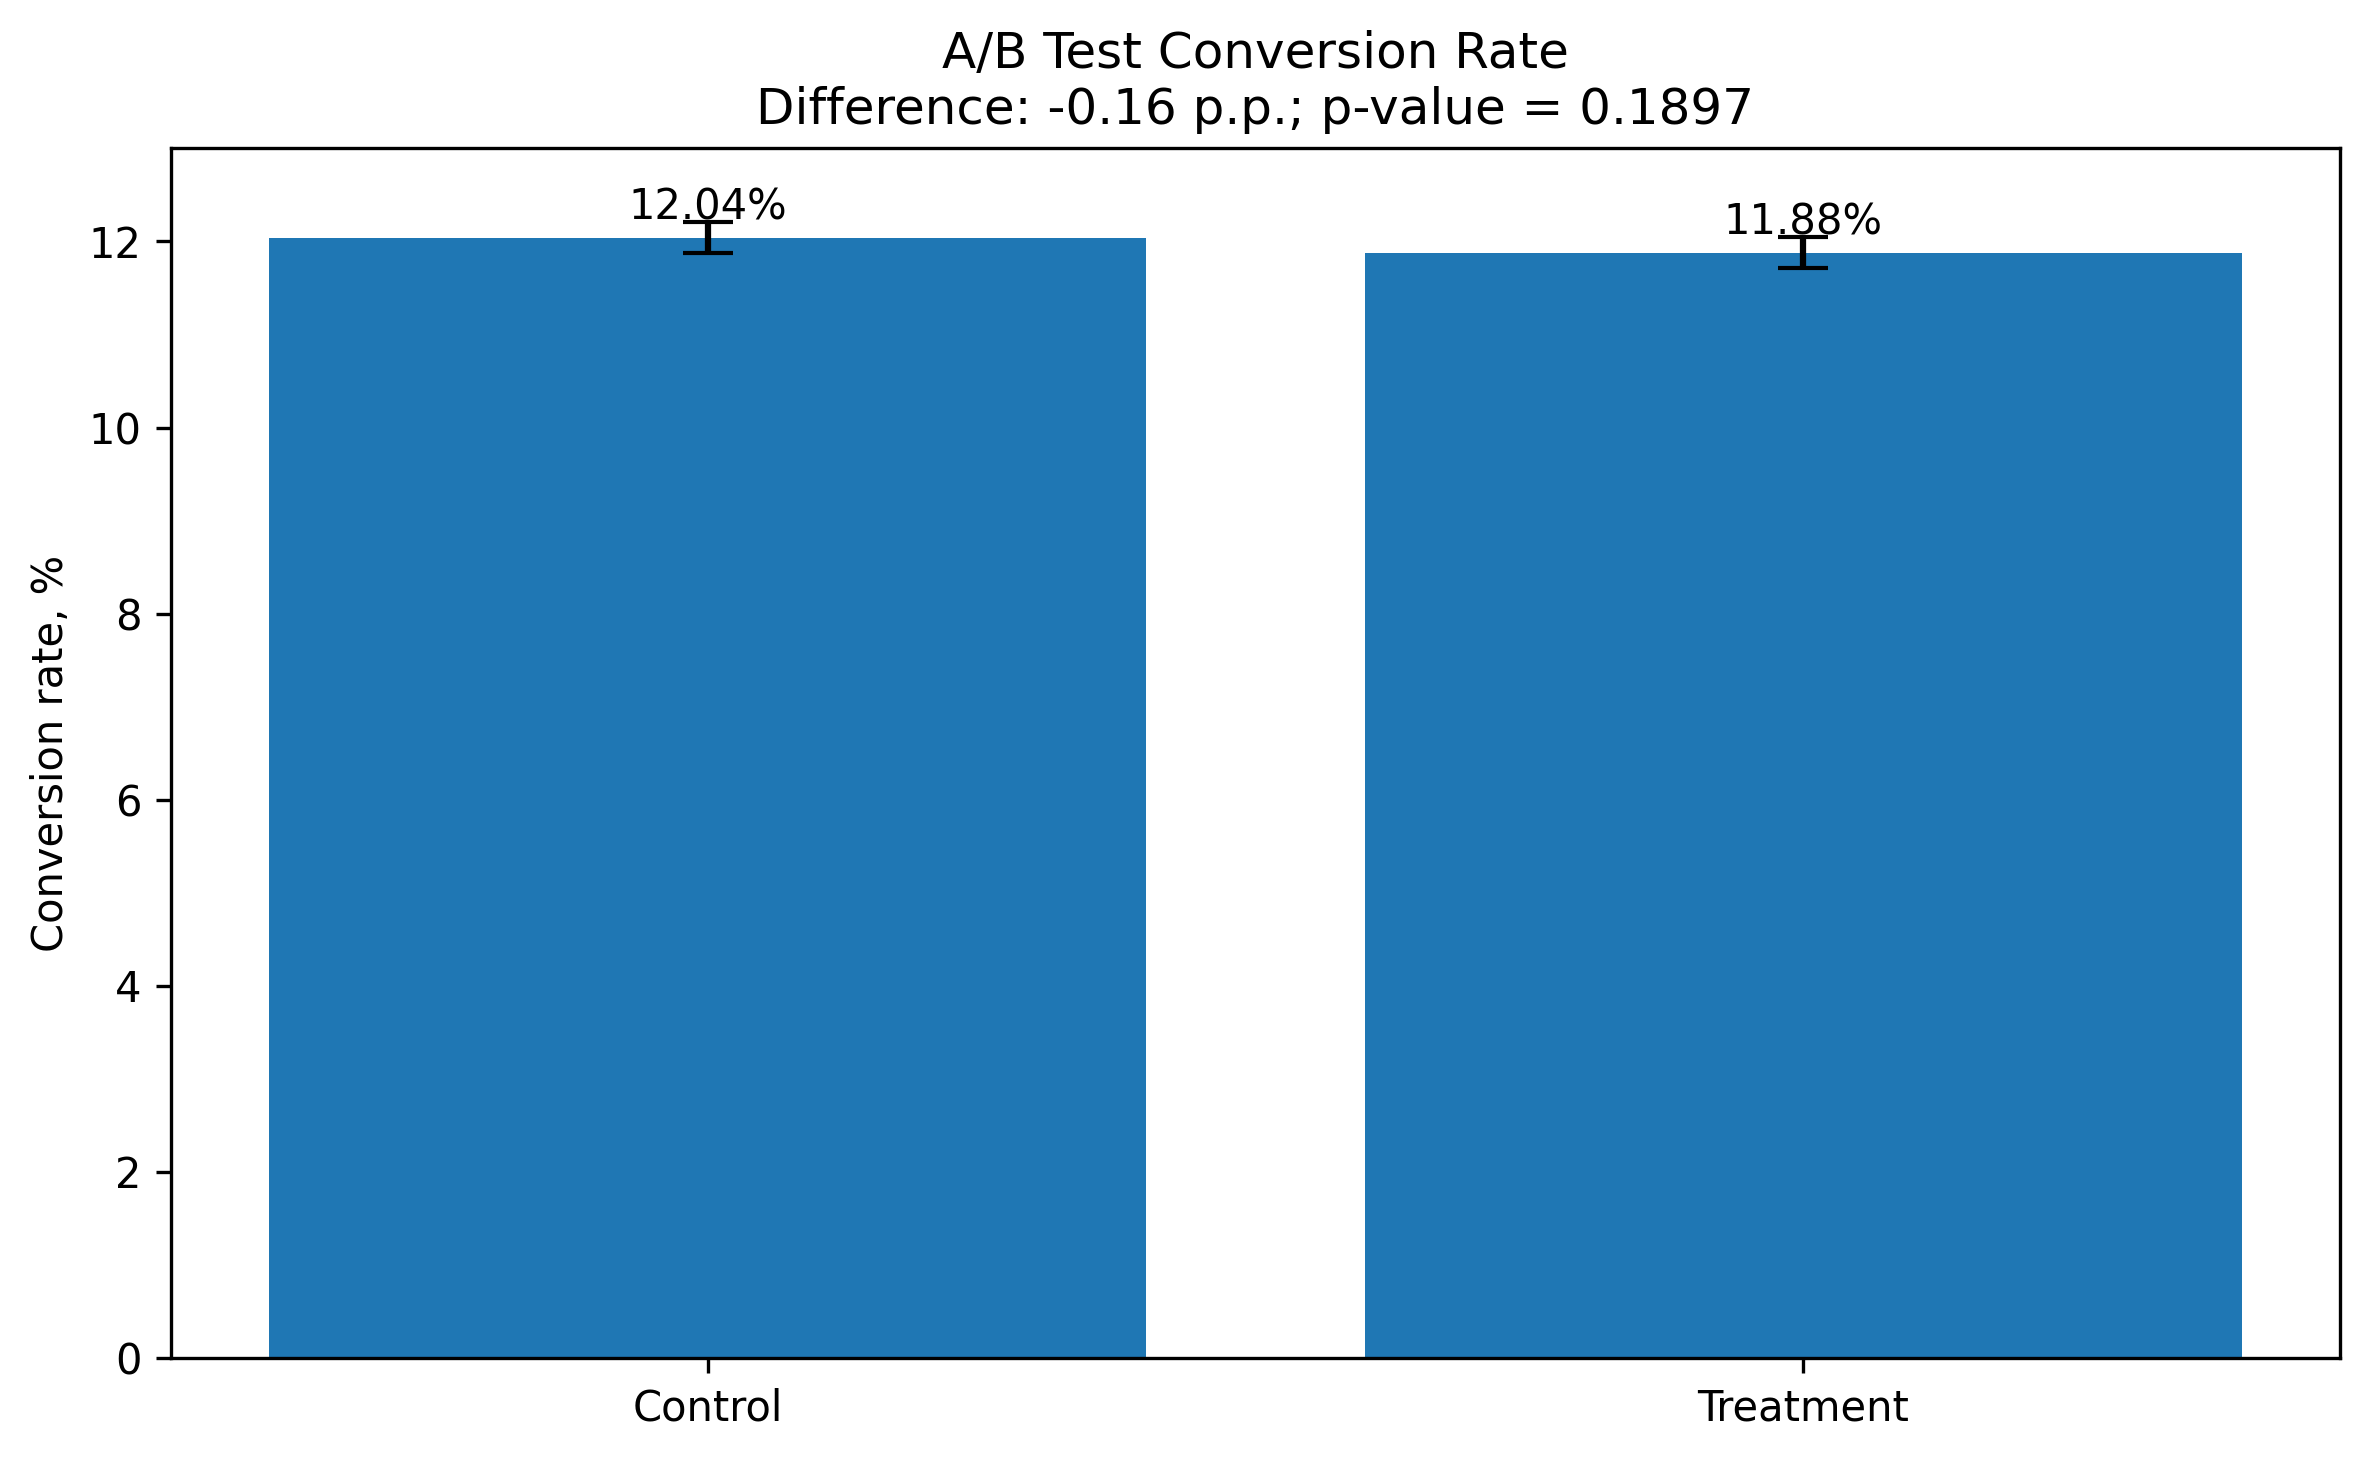
\includegraphics[
        width=0.65\textwidth
    ]{ab_test_conversion.png}
    \caption{Конверсия контрольной и тестовой групп}
\end{figure}

% ---------------------------------------------------------
\subsection{Проверка распределения пользователей}
% ---------------------------------------------------------

Перед сравнением конверсий была выполнена проверка Sample Ratio
Mismatch.

Ожидаемое распределение пользователей между группами составляло 50/50.

Результат проверки:

\[
p\text{-value}_{SRM}
=
0{,}9453.
\]

Значение значительно превышает 0,05. Признаков нарушения распределения
пользователей между группами не обнаружено.

% ---------------------------------------------------------
\subsection{Статистическая проверка}
% ---------------------------------------------------------

Результат z-теста:

\[
z = -1{,}3116,
\]

\[
p\text{-value} = 0{,}1897.
\]

Так как

\[
0{,}1897 > 0{,}05,
\]

нулевая гипотеза не отклоняется.

Статистически значимого различия между конверсиями контрольной и
тестовой групп не обнаружено.

95\%-й доверительный интервал для разницы конверсий:

\[
[-0{,}3939;\;0{,}0781]
\text{ п.п.}
\]

Интервал включает ноль. Реальный эффект может быть небольшим
отрицательным, практически нулевым или слабо положительным.

\newpage
% ---------------------------------------------------------
\subsection{Минимальный обнаруживаемый эффект}
% ---------------------------------------------------------

При уровне значимости 5\% и мощности 80\% эксперимент мог надёжно
обнаружить изменение примерно от:

\[
MDE = 0{,}3403
\text{ п.п.}
\]

В относительном выражении:

\[
MDE_{\text{relative}}
=
2{,}8266\%.
\]

Наблюдаемая разница составила только \(-0{,}1579\) процентного пункта,
что меньше рассчитанного MDE.

Это не доказывает полное отсутствие эффекта. Результат означает,
что эксперимент не обладал достаточной чувствительностью для
надёжного обнаружения настолько небольшого изменения.

% ---------------------------------------------------------
\subsection{Необходимый размер выборки}
% ---------------------------------------------------------

Для обнаружения наблюдаемой разницы при мощности 80\% потребовалось бы:

\begin{itemize}
    \item 662~801 пользователь в контрольной группе;
    \item 662~970 пользователей в тестовой группе;
    \item 1~325~770 пользователей всего.
\end{itemize}

Фактическая выборка составила 290~585 пользователей.

Для будущих экспериментов размер выборки следует рассчитывать заранее
на основе минимального бизнес-значимого эффекта, а не на основе
результата уже проведённого теста.

\newpage
% ---------------------------------------------------------
\section{Результаты A/B-теста по странам}
% ---------------------------------------------------------

Дополнительно результаты были проверены отдельно для Канады,
Великобритании и США.

\begin{table}[H]
    \centering
    \caption{Эффект новой страницы по странам}
    \begin{tabular}{lrrr}
        \toprule
        Страна &
        Control, \% &
        Treatment, \% &
        Разница, п.п. \\
        \midrule
        CA & 11,8783 & 11,1902 & -0,6881 \\
        UK & 12,0022 & 12,1171 &  0,1149 \\
        US & 12,0630 & 11,8464 & -0,2166 \\
        \bottomrule
    \end{tabular}
\end{table}

После применения поправки Холма статистически значимого эффекта
не обнаружено ни в одной стране.

\begin{figure}[H]
    \centering
    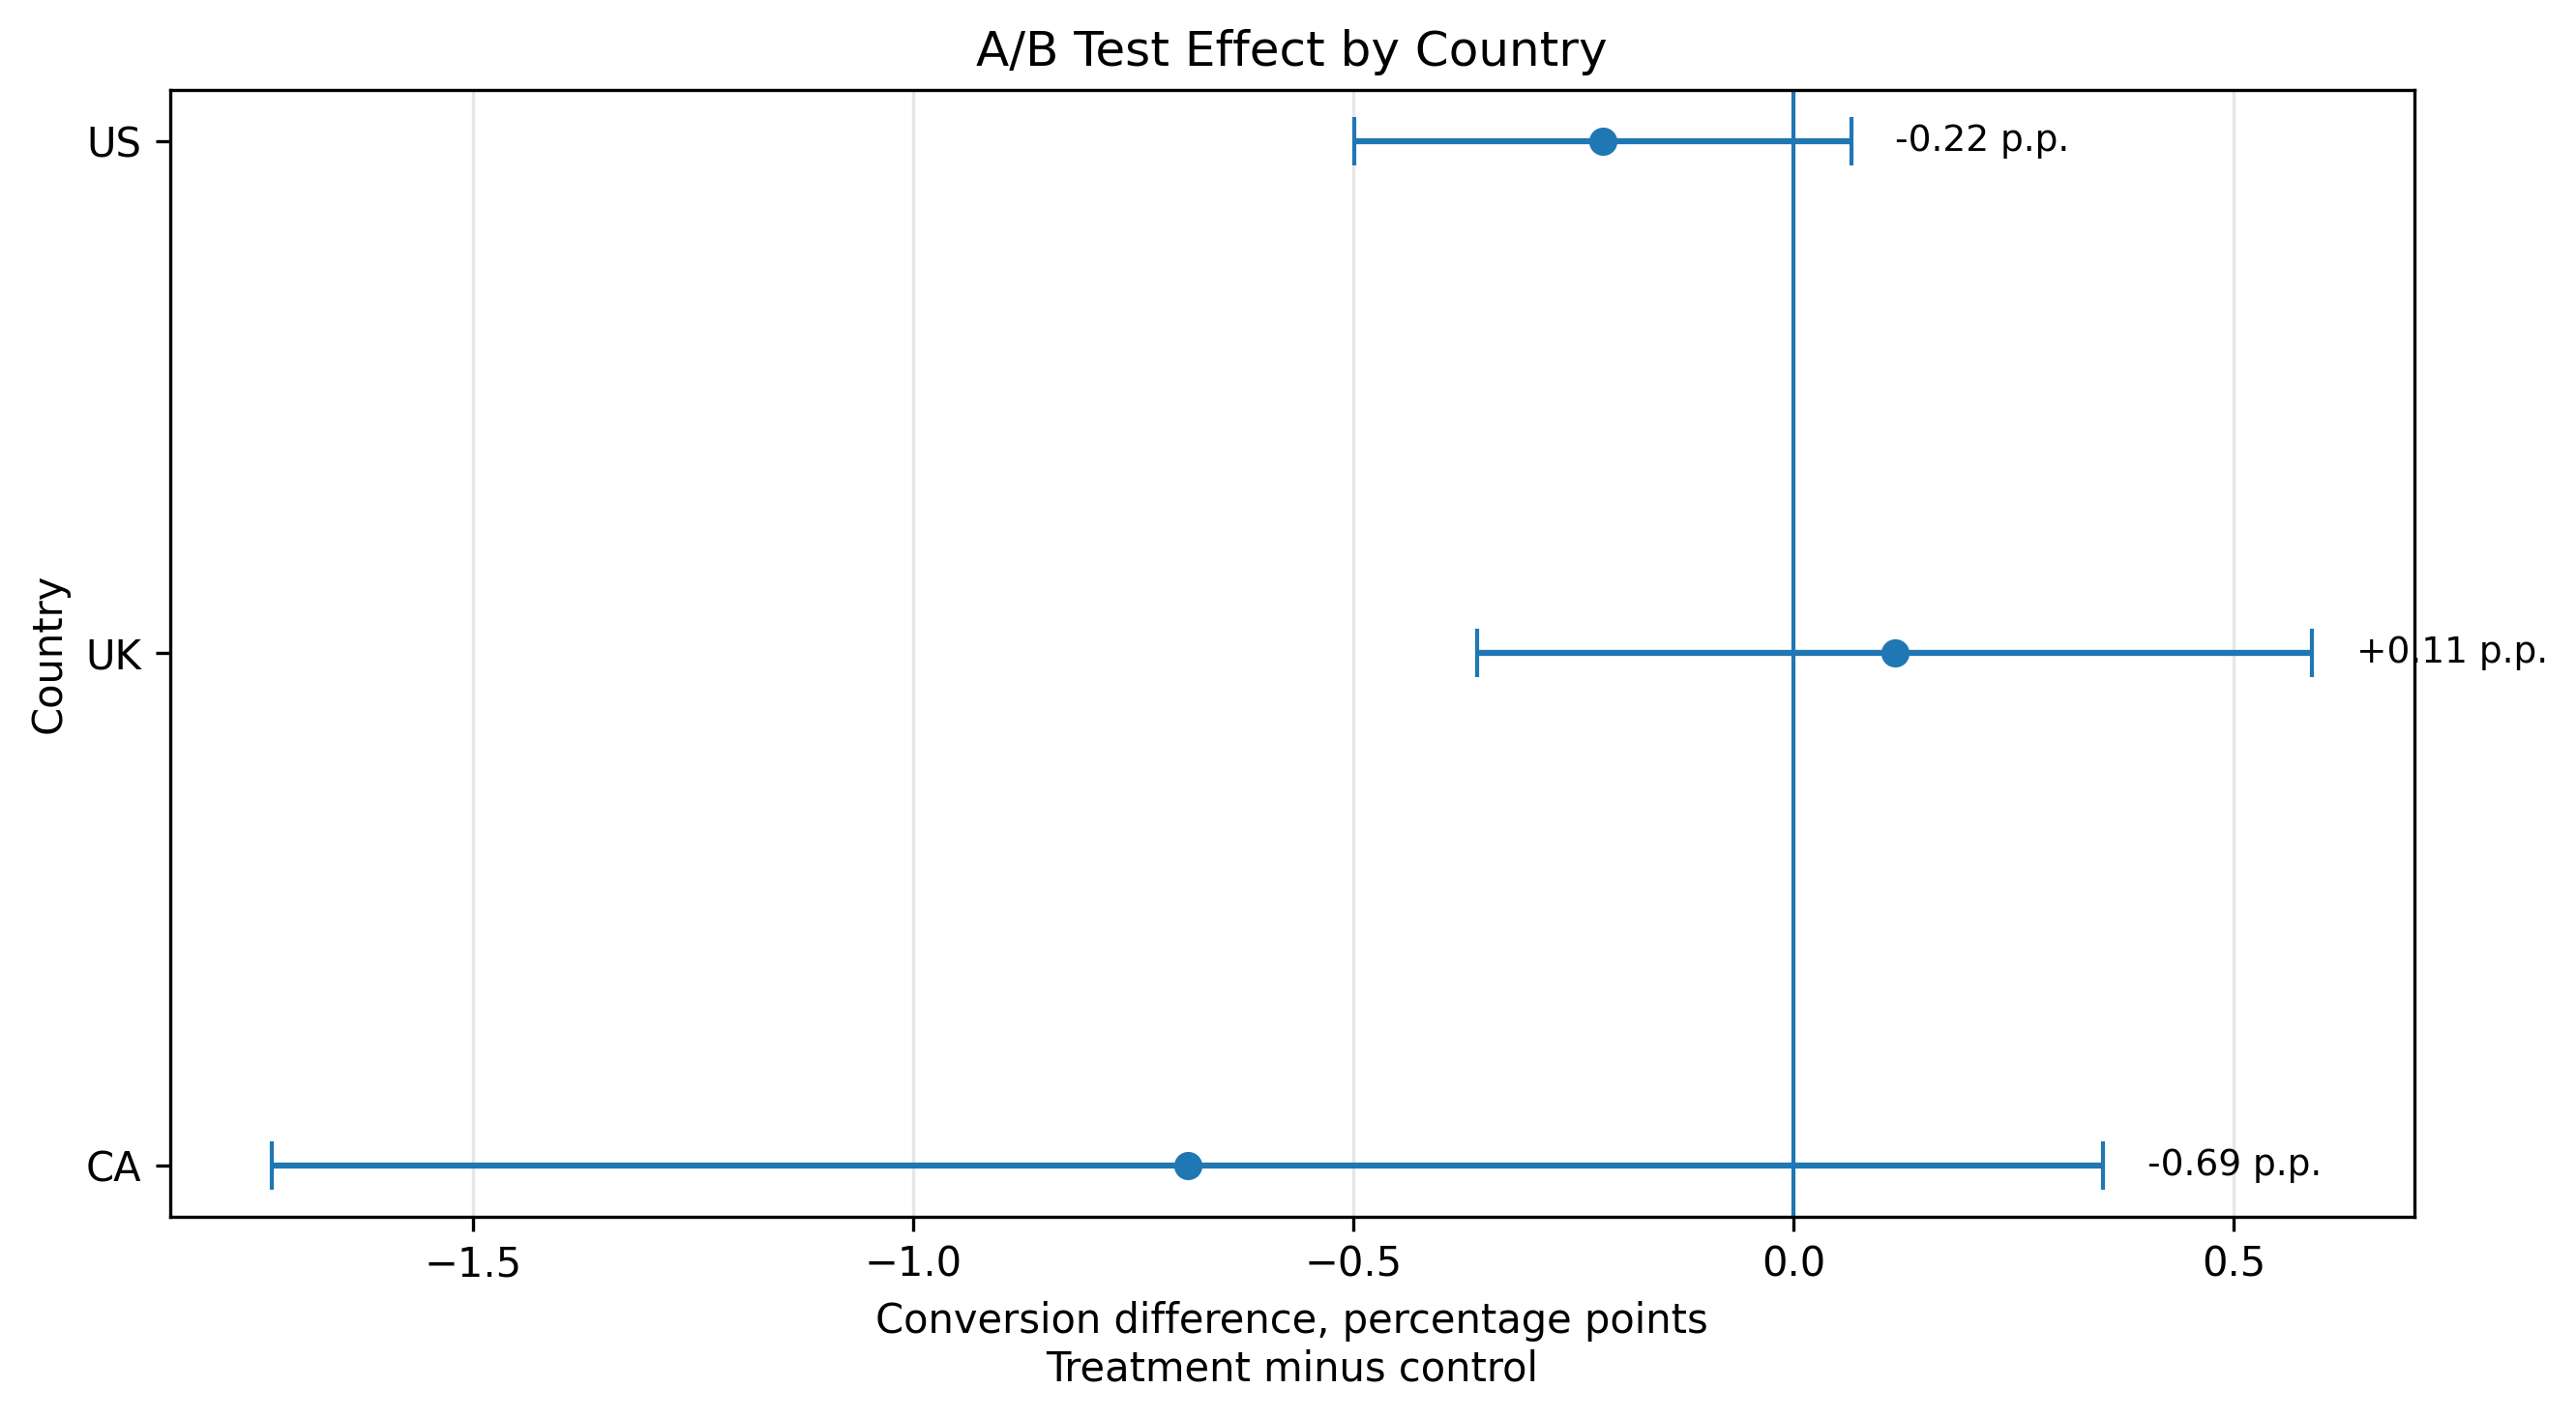
\includegraphics[
        width=0.75\textwidth
    ]{ab_test_effect_by_country.png}
    \caption{Эффект новой страницы по странам}
\end{figure}

Для проверки различий эффекта между странами использовался тест
Бреслоу--Дэя.

Результат:

\[
p\text{-value}
=
0{,}2915.
\]

Оснований считать, что эффект новой страницы статистически различается
между странами, нет.

Объединённое отношение шансов составило:

\[
OR = 0{,}9852,
\]

95\%-й доверительный интервал:

\[
[0{,}9633;\;1{,}0075].
\]

Интервал включает единицу, поэтому статистически подтверждённого
общего изменения шансов конверсии нет.

% ---------------------------------------------------------
\section{Итоговые выводы}
% ---------------------------------------------------------

По результатам анализа были получены следующие выводы:

\begin{enumerate}
    \item Ежемесячные продуктовые показатели в течение года были
    достаточно стабильными.

    \item Выручка находилась в диапазоне 5,59--6,35 млн в месяц.

    \item Месячные изменения выручки в большей степени связаны
    с количеством покупок, чем со средним чеком.

    \item Повторные покупатели составляют 71,1\% покупателей
    и формируют 88,1\% выручки.

    \item Медианное время до второй покупки составляет 81 день.

    \item Только 22,04\% повторных покупателей совершают вторую
    покупку в течение 30 дней.

    \item Ежемесячный когортный retention в большинстве случаев
    находится примерно на уровне 14--18\%.

    \item Новая страница показала конверсию на 0,1579 процентного
    пункта ниже контрольной.

    \item Полученная разница статистически незначима:
    \(p\text{-value}=0{,}1897\).

    \item Доверительный интервал включает ноль, поэтому доказательств
    влияния новой страницы на конверсию нет.

    \item Оснований внедрять новую страницу с целью повышения
    конверсии не обнаружено.

    \item Для будущих экспериментов необходимо заранее рассчитывать
    размер выборки на основе бизнес-значимого эффекта.
\end{enumerate}

\newpage
% ---------------------------------------------------------
\section{Ограничения анализа}
% ---------------------------------------------------------

К основным ограничениям относятся:

\begin{itemize}
    \item неполная временная метка в наборе A/B-теста;
    \item невозможность провести анализ динамики эксперимента по дням;
    \item отсутствие надёжной последовательной событийной воронки;
    \item большое число сессий только с одним событием;
    \item нестабильная связь идентификаторов товаров с категориями;
    \item признаки искусственно сгенерированных данных;
    \item правое цензурирование при анализе повторных покупок.
\end{itemize}

Несмотря на ограничения, набор данных позволяет продемонстрировать
полный цикл продуктового анализа: от проверки качества данных и
расчёта метрик до когортного анализа и статистической проверки
A/B-теста.


\end{document}